% \documentclass{jarticle}
\documentclass[openany]{report}
\setlength { \textheight } { 47\baselineskip }
\setlength { \textwidth } { 50zw }
\usepackage[top=25mm, bottom=25mm, left=18mm, right=18mm]{geometry}

\usepackage{amsmath}
\usepackage{ascmac}
\usepackage{bm}
\usepackage{booktabs}
\usepackage{comment}
\usepackage{fancybox}
\usepackage{fancyhdr}
\usepackage{hyperref}
\usepackage{here}
\usepackage{multicol}
\usepackage[dvipdfmx]{graphicx,color}
\usepackage{plext}
\usepackage{txfonts}

\makeindex

\begin{document}

\title{ \fontsize{60pt}{40pt}\selectfont SATOROOT}
\author{松本 悟}
\maketitle

\pagestyle{fancy}
\fancyhead{}
\fancyhead[RO,RE]{\rightmark}
\fancyhead[LE,LO]{\leftmark}
\cfoot{\thepage} 

% \renewcommand{\chaptermark}[1]{\markboth{第\ \thechapter\ 章~#1}{}}
\renewcommand{\sectionmark}[1]{\markright{\thesection \ \ #1}{}}

\newcommand{\ROOT}{\texttt{ROOT}}
\newcommand{\Cpp}{\texttt{C++}}


\pagenumbering{roman}

\clearpage
\setcounter{section}{-1} % 章数をゼロから始めます。
%%%%%%%%%%%%%%%%%%%%%%%%%%%%%%%%%%%%%%%%%%%%%%%%%%%%%%%%%%%%%%%%%%%%%%%%%%%%%%%%%
%%        %%%        %%%        %%%        %%%        %%%         %%%  %%%%  %%%
%%  %%%%%%%%%  %%%%%%%%%  %%%%%%%%%%%%  %%%%%%%%%  %%%%%%  %%%%%  %%%    %%  %%%
%%        %%%        %%%  %%%%%%%%%%%%  %%%%%%%%%  %%%%%%  %%%%%  %%%  %  %  %%%
%%%%%%%%  %%%  %%%%%%%%%  %%%%%%%%%%%%  %%%%%%%%%  %%%%%%  %%%%%  %%%  %%    %%%
%%        %%%        %%%        %%%%%%  %%%%%%        %%%         %%%  %%%   %%%
%%%%%%%%%%%%%%%%%%%%%%%%%%%%%%%%%%%%%%%%%%%%%%%%%%%%%%%%%%%%%%%%%%%%%%%%%%%%%%%%%
 \section{前書き}


  \subsection{どんな人向け}
  \begin{itemize}
   \item 実験系の研究室に配属されてデータの解析をする段階になった人
   \item 先輩に「 \ROOT 使えるようになっといてね」とか言われちゃった人
  \end{itemize}
  そんな人の為の覚え書き。
  SATOROOTとは、本ドキュメントの前身を私の後輩が作業する為に作成していたディレクトリ名から拝借した名前である。


  \subsection{方針}
  とりあえず動かす。
  \Cpp の細かいお作法とか正しい言葉の使い方とかは無視。
  とりあえず動かす上で必要なお作法やおまじないについてはその都度紹介したりしなかったりする。
  とにかく動かせるようにすることを目指す。
  ただし、自分で調べることにも重きを置くのでサンプルを示したらその都度サンプルをいじる練習問題を提供する。


  \subsection{作業環境}
  著者の作業環境は
  \begin{enumerate}
   \item 
	 \verb|OS X 10.8.5|
   \item 
	 \verb|ROOT version 5.34/09|
  \end{enumerate}


  \subsection{お約束事}
  \begin{enumerate}
   \item \verb|$| \ --- \ プロンプトを表す記号。パソコンがユーザーの入力を受け入れる状態を表す。
   \item \verb|root[i]| \ --- \ \verb|i|には数字が入る。
	 コマンドライン上で\ROOT を作業している時の行番号である。
	 \verb|i|を省略することもある。
   \item \verb|SATOROOT| \ --- \ この覚え書きで使用する全てのファイルは\verb|SATOROOT|以下のディレクトリで行う。
  \end{enumerate}


\tableofcontents

\chapter{マクロを使う}
\pagenumbering{arabic}
\setcounter{page}{1}


%%%%%%%%%%%%%%%%%%%%%%%%%%%%%%%%%%%%%%%%%%%%%%%%%%%%%%%%%%%%%%%%%%%%%%%%%%%%%%%%%
%%        %%%        %%%        %%%        %%%        %%%         %%%  %%%%  %%%
%%  %%%%%%%%%  %%%%%%%%%  %%%%%%%%%%%%  %%%%%%%%%  %%%%%%  %%%%%  %%%    %%  %%%
%%        %%%        %%%  %%%%%%%%%%%%  %%%%%%%%%  %%%%%%  %%%%%  %%%  %  %  %%%
%%%%%%%%  %%%  %%%%%%%%%  %%%%%%%%%%%%  %%%%%%%%%  %%%%%%  %%%%%  %%%  %%    %%%
%%        %%%        %%%        %%%%%%  %%%%%%        %%%         %%%  %%%   %%%
%%%%%%%%%%%%%%%%%%%%%%%%%%%%%%%%%%%%%%%%%%%%%%%%%%%%%%%%%%%%%%%%%%%%%%%%%%%%%%%%%
 \section{\ROOT}


  \subsection{\ROOT とは}
  \ROOT ( \url{http://root.cern.ch/drupal/} ) とは、
  高エネルギー業界で広く普及している膨大なデータを効率的に扱うためのフレームワークです。
  \Cpp のお作法でプログラミングします。
  コマントライン上で\ROOT と対話的にプロットやプログラミングを行うことが出来ます。


  \subsection{なぜ\ROOT }
  世の中のいろんなニーズに応えた結果です。(投げやり)


  \subsection{\ROOT のインストール}
  \ROOT のインストール作業を行う。
  \begin{itemize}
   \item \texttt{/usr/local/hep/root/5.34.09} \ --- \ \ROOT のライブラリ置き場
   \item \texttt{~/tmp} \ --- \ コンパイルを実行する時の場所
  \end{itemize}


   \subsubsection*{各ディレクトリの作成}
\begin{verbatim}
	$ sudo mkdir -p /usr/local/hep/root/v5.34.09
	$ mkdir ~/tmp
\end{verbatim}


   \subsubsection*{\ROOT のソースコードのダウンロードと展開}
\begin{verbatim}
	$ cd ~/tmp
	$ sudo wget ftp://root.cern.ch/root/root_v5.34.09.source.tar.gz
	$ ls
	root_v5.34.09.source.tar.gz
	$ sudo tar zxvf root_v5.34.09.source.tar.gz
	$ ls
	root
	root_v5.34.09.source.tar.gz
\end{verbatim}


   \subsubsection*{環境変数の定義}
\begin{verbatim}
	$ export ROOTSYS=/usr/local/hep/root/v5.34.09
\end{verbatim}


   \subsubsection*{インストール作業}
\begin{verbatim}
	$ cd root
	$ sudo ./configure --prefix=/usr/local/hep/root/v5.34.09
\end{verbatim}
以下のコメントが出てくると\texttt{configure}は成功
\begin{verbatim}
	To build ROOT type:

	make
	make  install
\end{verbatim}
指示に従い、
\verb|make|及び\verb|make install|を行う。
コンパイルする。
\begin{verbatim}
	$ make
\end{verbatim}
以下のコメントが出てくると\texttt{make}は成功
\begin{verbatim}
	============================================================
	===                ROOT BUILD SUCCESSFUL.                ===
	=== Run 'make install' now.                              ===
	============================================================
\end{verbatim}
インストールする。
\begin{verbatim}
	$ su
	Password:
	$ make install
	...
	$ exit
\end{verbatim}


   \subsubsection*{一時ファイルの削除}
\begin{verbatim}
	$ cd ../
	$ pwd
	/tmp
	$ rm -rf root
\end{verbatim}


   \subsubsection*{環境変数ファイルの作成}
   \ROOT 用の環境変数定義を書き込んだ\verb|setup.sh|を準備して、
   ホームディレクトリに置く。
   \begin{itembox}{\texttt{setup.sh}}
\begin{verbatim}
	export ROOTSYS=/usr/local/hep/root/v5.34.09
	export PATH=${ROOTSYS}/bin:${PATH} 
	export LD_LIBRARY_PATH=${ROOTSYS}/lib/root:${LD_LIBRARY_PATH}
\end{verbatim}
   \end{itembox}
   ホームディレクトリ内のファイル\verb|.bash_profile|に以下の一文を追加する。
\begin{verbatim}
	source /usr/local/hep/root/setup.sh
\end{verbatim}
その後、
\begin{verbatim}
	source .bash_profile
\end{verbatim}
 
\clearpage

%%%%%%%%%%%%%%%%%%%%%%%%%%%%%%%%%%%%%%%%%%%%%%%%%%%%%%%%%%%%%%%%%%%%%%%%%%%%%%%%%
%%        %%%        %%%        %%%        %%%        %%%         %%%  %%%%  %%%
%%  %%%%%%%%%  %%%%%%%%%  %%%%%%%%%%%%  %%%%%%%%%  %%%%%%  %%%%%  %%%    %%  %%%
%%        %%%        %%%  %%%%%%%%%%%%  %%%%%%%%%  %%%%%%  %%%%%  %%%  %  %  %%%
%%%%%%%%  %%%  %%%%%%%%%  %%%%%%%%%%%%  %%%%%%%%%  %%%%%%  %%%%%  %%%  %%    %%%
%%        %%%        %%%        %%%%%%  %%%%%%        %%%         %%%  %%%   %%%
%%%%%%%%%%%%%%%%%%%%%%%%%%%%%%%%%%%%%%%%%%%%%%%%%%%%%%%%%%%%%%%%%%%%%%%%%%%%%%%%%
 \section{\ROOT をコマンドラインで使う}


  \subsection{\ROOT を起動する}
\begin{verbatim}
	$ root
\end{verbatim}
\ROOT の起動画面が立ち上がり、
\begin{figure}[htbp]
 \begin{center}
  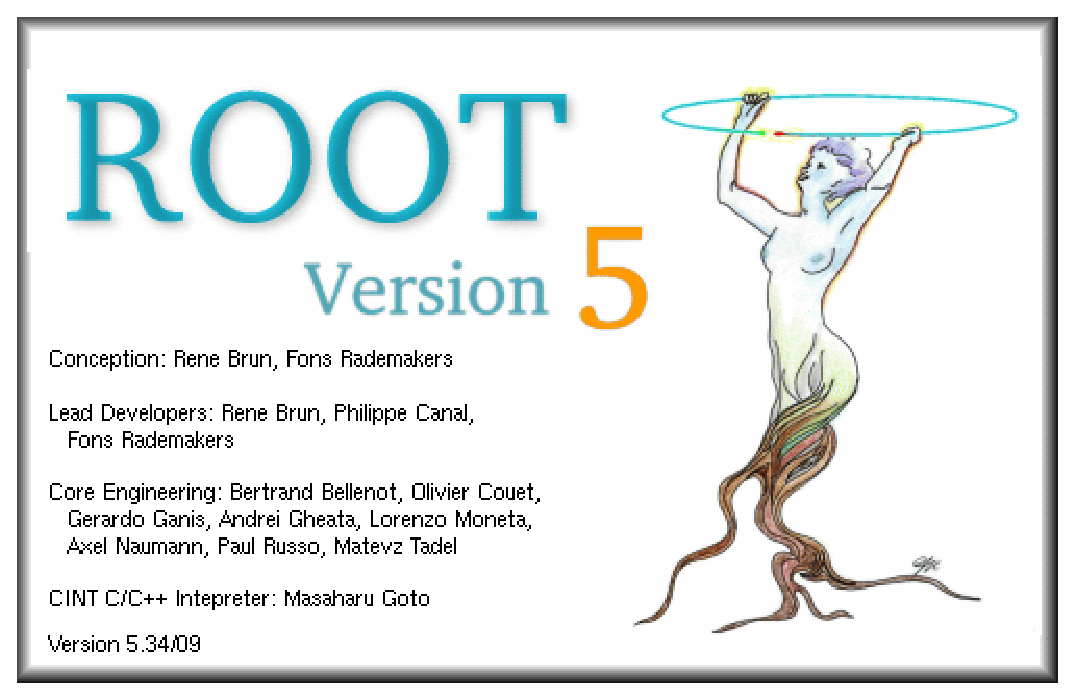
\includegraphics[width = 80mm]{./picture/root_starting.eps}
 \end{center}
 \caption{\ROOT の起動画面}
 \label{Fig:root_starting}
\end{figure}
\begin{verbatim}
	*******************************************
	*                                         *
	*        W E L C O M E  to  R O O T       *
	*                                         *
	*   Version   5.34/09      26 June 2013   *
	*                                         *
	*  You are welcome to visit our Web site  *
	*          http://root.cern.ch            *
	*                                         *
	*******************************************

	ROOT 5.34/09 (v5-34-09@v5-34-09, Jun 26 2013, 17:10:36 on macosx64)

	CINT/ROOT C/C++ Interpreter version 5.18.00, July 2, 2010
	Type ? for help. Commands must be C++ statements.
	Enclose multiple statements between { }.
\end{verbatim}
という一連の情報が表示された後、
\begin{verbatim}
	root[0]
\end{verbatim}
となって\ROOT が立ち上がり操作可能になる。

   \subsubsection{\ROOT の起動画面を省略する}
   \verb|root|起動時に\verb|-l|オプションをつければ起動画面は省略される。
\begin{verbatim}
	$ root -l
\end{verbatim}

   \subsubsection{\ROOT の起動画面を常に省略する}
   いちいち \verb|-l| オプションをつけるのが面倒くさい人はbash起動時に自動的に読み込まれるファイル \verb|~/.bash_profile| に次の文章を追加する。
\begin{verbatim}
	alias root="root -l"
\end{verbatim}
次に\verb|source|コマンドを使用すればよい。
\begin{verbatim}
	$ source ~/.bash_profile
\end{verbatim}


この状態でも\ROOT の起動画面を省略しない場合には
\begin{verbatim}
	$ \root 
\end{verbatim}

   \subsubsection{\ROOT がデフォルトで読み込むファイル}

  \subsection{\ROOT を終了する}

\begin{verbatim}
	root[] .q
\end{verbatim}

\clearpage
%%%%%%%%%%%%%%%%%%%%%%%%%%%%%%%%%%%%%%%%%%%%%%%%%%%%%%%%%%%%%%%%%%%%%%%%%%%%%%%%%
%%        %%%        %%%        %%%        %%%        %%%         %%%  %%%%  %%%
%%  %%%%%%%%%  %%%%%%%%%  %%%%%%%%%%%%  %%%%%%%%%  %%%%%%  %%%%%  %%%    %%  %%%
%%        %%%        %%%  %%%%%%%%%%%%  %%%%%%%%%  %%%%%%  %%%%%  %%%  %  %  %%%
%%%%%%%%  %%%  %%%%%%%%%  %%%%%%%%%%%%  %%%%%%%%%  %%%%%%  %%%%%  %%%  %%    %%%
%%        %%%        %%%        %%%%%%  %%%%%%        %%%         %%%  %%%   %%%
%%%%%%%%%%%%%%%%%%%%%%%%%%%%%%%%%%%%%%%%%%%%%%%%%%%%%%%%%%%%%%%%%%%%%%%%%%%%%%%%%
 \section{\ROOT でマクロを読む/実行する方法}
 \ROOT への命令文が書かれたプログラムのソースコード\verb|hello.cpp|を準備しよう。
 今はソースコードを理解しなくてもいいが、
 気になる人は付録\ref{sec:namespace}などを参考にして理解せよ。
 \begin{itembox}{\texttt{hello.cpp}}
\begin{verbatim}
	#include <iostream>
	void hello(){
	std::cout << "Hello, world" << std::endl ;
	}
\end{verbatim}
 \end{itembox}

  \subsection{\texttt{hello.cpp}の実行方法1}
  \verb|hello.cpp|を\ROOT 起動時に実行するには、
\begin{verbatim}
	$ root hello.cpp
\end{verbatim}
上記のコマンドを実行すると、
\begin{verbatim}
	root [0] 
	Processing hello.cpp...
	Hello, World
\end{verbatim}

  \subsection{\texttt{hello.cpp}の実行方法2}
  別の方法は\ROOT をいったん起動して、プログラムを"ロード"して実行するという手段。
\begin{verbatim}
	$ root
	root [0] .L hello.cpp 
	root [1] hello()
	Hello, World
\end{verbatim}

  \subsection{\texttt{hello.cpp}の実行方法3(推奨)}
  ロードする時に\Cpp コンパイラを通してマクロに含まれるエラーメッセージなどを表記してくれる方法。
  やり方は'\verb|+|'をロードするファイル名の末尾につける。
  ( \url{http://root.cern.ch/drupal/content/compiling-macros} )
\begin{verbatim}
	$ root
	root [0] .L hello.cpp+
\end{verbatim}

例えば\verb|hello.cpp|の\verb|std::endl;|のセミコロンが無い時にはどうなるかというと、
下のようにエラーメッセージと何が悪いのかをコンパイラが返してくれる。
\begin{verbatim}
	Info in <TUnixSystem::ACLiC>: creating shared library /Users/SATOROOT/hello_cpp.so
	In file included from /Users/SATOROOT/hello_cpp_ACLiC_dict.cxx:17:
	In file included from /Users/SATOROOT/hello_cpp_ACLiC_dict.h:34:
	/Users/SATOROOT/hello.cpp:3:42: error: expected ';' after expression
	std::cout << "Hello, World" <<std::endl 
	^
	;
	In file included from /Users/SATOROOT/hello_cpp_ACLiC_dict.cxx:17:
	In file included from /Users/SATOROOT/hello_cpp_ACLiC_dict.h:18:
	/usr/local/hep/root/v5.34.09/include/root/G__ci.h:971:7:  \
	warning: private field 'type' is not used [-Wunused-private-field]
	int type;
	^
	/usr/local/hep/root/v5.34.09/include/root/G__ci.h:972:7: \
	warning: private field 'tagnum' is not used [-Wunused-private-field]
	int tagnum;
	^
	/usr/local/hep/root/v5.34.09/include/root/G__ci.h:973:7: \
	warning: private field 'typenum' is not used [-Wunused-private-field]
	int typenum;
	^
	/usr/local/hep/root/v5.34.09/include/root/G__ci.h:975:19: warning: \
	private field 'isconst' is not used
	[-Wunused-private-field]
	G__SIGNEDCHAR_T isconst;
	^
	/usr/local/hep/root/v5.34.09/include/root/G__ci.h:977:29: warning: \
	private field 'dummyForCint7' is not used
	[-Wunused-private-field]
	struct G__DUMMY_FOR_CINT7 dummyForCint7;
	^
	5 warnings and 1 error generated.
	clang: error: no such file or directory: '/Users/SATOROOT/hello_cpp_ACLiC_dict.o'
	Error in <ACLiC>: Compilation failed!
\end{verbatim}
\clearpage
%%%%%%%%%%%%%%%%%%%%%%%%%%%%%%%%%%%%%%%%%%%%%%%%%%%%%%%%%%%%%%%%%%%%%%%%%%%%%%%%
%%        %%%        %%%        %%%        %%%        %%%         %%%  %%%%  %%%
%%  %%%%%%%%%  %%%%%%%%%  %%%%%%%%%%%%  %%%%%%%%%  %%%%%%  %%%%%  %%%    %%  %%%
%%        %%%        %%%  %%%%%%%%%%%%  %%%%%%%%%  %%%%%%  %%%%%  %%%  %  %  %%%
%%%%%%%%  %%%  %%%%%%%%%  %%%%%%%%%%%%  %%%%%%%%%  %%%%%%  %%%%%  %%%  %%    %%%
%%        %%%        %%%        %%%%%%  %%%%%%        %%%         %%%  %%%   %%%
%%%%%%%%%%%%%%%%%%%%%%%%%%%%%%%%%%%%%%%%%%%%%%%%%%%%%%%%%%%%%%%%%%%%%%%%%%%%%%%%
 \section{幾つかの常套手段}
 
 
  \subsection{引数を数字にする}
  引数としてある整数を与えて、
  その数自身、その数の二乗、その数の三乗を出力するサンプルプログラムが\verb|usual1.cpp|である。
  \begin{itembox}{\texttt{usual1.cpp}}
\begin{verbatim}
#include <iostream>
#include "TMath.h"
void usual1(int i){
  std::cout << i << std::endl ;
  std::cout << TMath::Power(i,2) << std::endl ;
  std::cout << TMath::Power(i,3) << std::endl ;
}
\end{verbatim}
  \end{itembox}
実行方法は次の通りである。
\begin{verbatim}
$ root
root [0] .L usual1.cpp+
root [1] usual1(3)
3
9
27
\end{verbatim}
なお、\verb|#include "TMath.h"|という命令文によって、
\ROOT に組み込まれている定数や数式演算を使用可能にしている。
\url{http://root.cern.ch/root/html/TMath.html}


  \subsection{引数を文字列にする}
  引数を文字列にしたい場合には
  \begin{itembox}{\texttt{usualchar.cpp}}
\begin{verbatim}
#include <iostream>
void usualchar(char *name){
  std::cout << "character string = " << name  << std::endl ;
}
\end{verbatim}
  \end{itembox}
実行方法は次の通りである。
\begin{verbatim}
$ root
root [0] .L usualchar.cpp 
root [1] usualchar("test")
character string = test
\end{verbatim}


  \subsection{引数を複数にする}
  複数個の引数を与えたい時には引数の\verb|()|の中に、
  \verb|,|を挟んで定義すれば良い。
  \begin{itembox}{\texttt{usualage.cpp}}
\begin{verbatim}
#include <iostream>
void usualage(char *name,int i){
  std::cout << name << " is " << i << "years old." << std::endl ;
}
\end{verbatim}
  \end{itembox}
実行方法は次の通りである。
\begin{verbatim}
$ root
root [0] .L usualage.cpp 
root [1] usualage("satoru",24)
satoru is 24years old.
\end{verbatim}
\clearpage
%%%%%%%%%%%%%%%%%%%%%%%%%%%%%%%%%%%%%%%%%%%%%%%%%%%%%%%%%%%%%%%%%%%%%%%%%%%%%%%%%
%%        %%%        %%%        %%%        %%%        %%%         %%%  %%%%  %%%
%%  %%%%%%%%%  %%%%%%%%%  %%%%%%%%%%%%  %%%%%%%%%  %%%%%%  %%%%%  %%%    %%  %%%
%%        %%%        %%%  %%%%%%%%%%%%  %%%%%%%%%  %%%%%%  %%%%%  %%%  %  %  %%%
%%%%%%%%  %%%  %%%%%%%%%  %%%%%%%%%%%%  %%%%%%%%%  %%%%%%  %%%%%  %%%  %%    %%%
%%        %%%        %%%        %%%%%%  %%%%%%        %%%         %%%  %%%   %%%
%%%%%%%%%%%%%%%%%%%%%%%%%%%%%%%%%%%%%%%%%%%%%%%%%%%%%%%%%%%%%%%%%%%%%%%%%%%%%%%%%
 \section{関数を描く}
 早速、関数を\ROOT で関数を描こう。
 \verb|sinfunction.cpp|を見てほしい。
 \begin{itembox}{\texttt{sinfunction.cpp}}
\begin{verbatim}
	#include "TF1.h"
	#include "TMath.h"
	TF1 *sinfunction(){
	  TF1 *f = new TF1("f","TMath::Sin(x)") ;
	  f->Draw() ;
	  return f ;
	}
\end{verbatim}
 \end{itembox}
 そしてとりあえず実行して欲しい。
\begin{verbatim}
	$ root
	root [0] .L sinfunction.cpp+
	root [1] sinfunction()
	Info in <TCanvas::MakeDefCanvas>:  created default TCanvas with name c1
	(class TF1*)0x7fe64437b580
\end{verbatim}
\begin{figure}[htbp]
 \begin{center}
  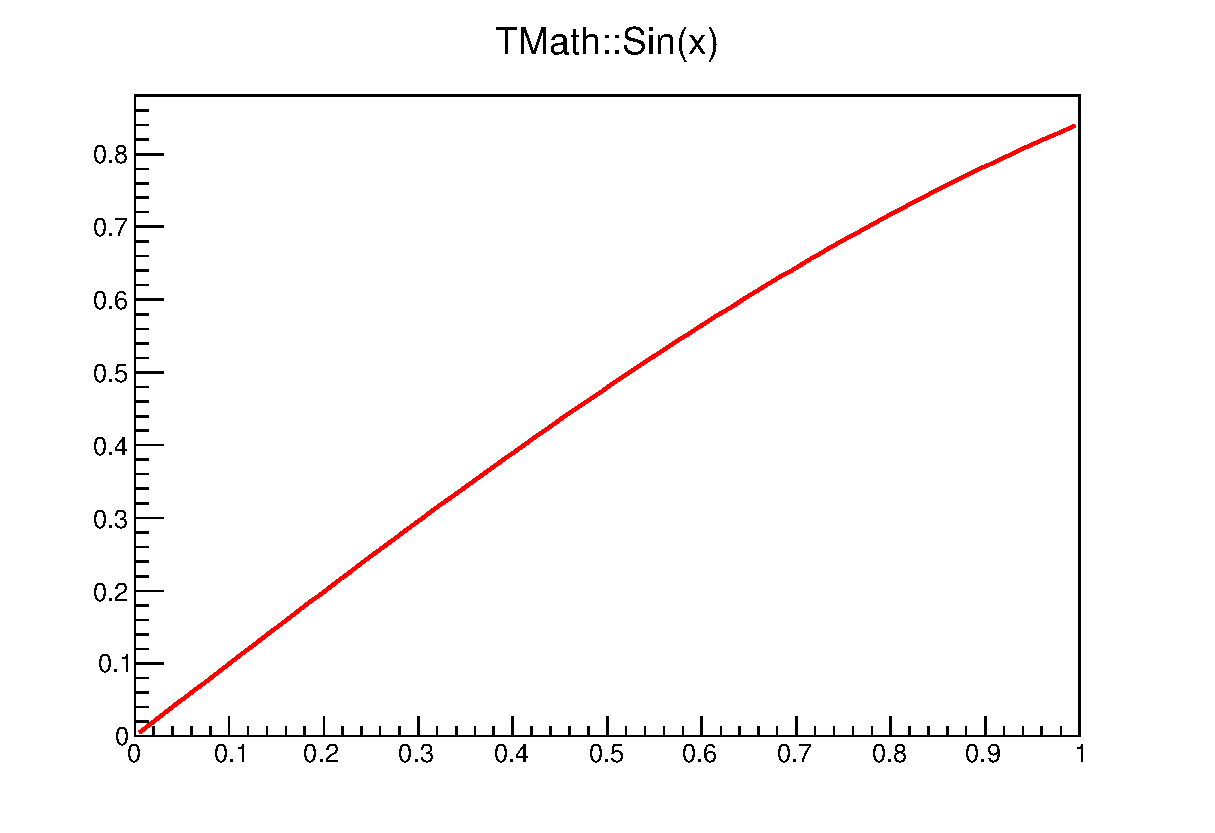
\includegraphics[width = 100mm]{./picture/sinfunctioncanvas1.eps}
 \end{center}
 \caption{\texttt{sinfunction.cpp}の実行結果}
 \label{Fig:sinfunctioncanvas1}
\end{figure}
おそらく、思っていたような定義域でない、軸に名前がついていないなどいろいろな不満があるだろう。
それらは全て人間が指定してあげる必要がある。
そういった手法も紹介していく。



これまであまりにすっ飛ばしてきたので、\verb|sinfunction.cpp|を一行目から簡単に見ていこう。
(\Cpp のお作法をしっかり学ぶつもりは無いので説明はそれなりの質なので気になる箇所は自分でググるべし)
\begin{enumerate}
 \item \verb|#include "TF1.h"| \\
       \ROOT で関数を描く為に必要となるライブラリ\verb|"TF1.h"|を読み込むという意味
 \item \verb|#include "TMath.h"| \\ 
       \ROOT で特定の定数$\pi$や$e$などの値や、
       関数$\sin(x)$、$\exp(x)$などを使用する時に必要となるライブラリ\verb|"TMath.h"|を読み込む。
 \item \verb|TF1 *sinfunction(){ |\\
       マクロの名前を準備するかを記述している箇所である。
       <型名> = \verb|TF1|、<関数名>=\verb|sinfunction|、<引数>=無し、を表している。
       \verb|*sinfunction|というのは\verb|sinfunction|という関数のポインタを意味するが、これ以上は触れない。
 \item \verb|TF1 *f = new TF1("f","TMath::Sin(x)") ;| \\
       ここからが\verb|sinfunction.cpp|の本文。
       この行の左辺では\verb|"TF1"|という型のポインタ\verb|f|を定義している。
       \verb|new|とは\Cpp のお作法でメモリを動的に確保する為のものである。
       \verb|TF1("f","TMath::Sin(x)")|とは左辺で定義した\verb|f|というポインタの名前を\verb|f|として、
       その間数は\verb|TMath|というライブラリの中で定義された\verb|Sin(x)|という関数にするという意味。
 \item \verb|f->Draw() ;| \\
       \verb|f|というポインタを描く。
       4行目のやり方で定義されたポインタ\verb|f|に対して命令を与える時には\verb|->|というアロー演算子を用いる。
 \item \verb|return f ;|
 \item \verb|}| \\
       3行目の\verb|{|に対応する括弧。
\end{enumerate}


  \subsection{練習}
  \begin{enumerate}
   \item 定義域を$-\pi$から$\pi$に変更せよ。
	 \begin{description}
	  \item[ヒント]  \url{http://root.cern.ch/root/html/TF1.html#TF1:TF1@1}
	 \end{description}
   \item $2\sin(x/2)$を描け。
	 \begin{description}
	  \item[ヒント]  \url{http://root.cern.ch/root/html/TF1.html#TopOfPage} の
		     B - Expression using variable x with parameters
	  \item[ヒント]\url{http://root.cern.ch/root/html/TFormula.html#TFormula:SetParameter}
	 \end{description}
   \item $ \sin(x) $と$ \cos(x) $を一緒に描け。
	 また$\sin(x)$の線を赤色、$\cos(x)$の線を緑色にせよ。
	 \begin{description}
	  \item[ヒント]  \url{http://root.cern.ch/root/html/TF1.html#TF1:Draw}
	  \item[ヒント]  \url{http://root.cern.ch/root/html/TAttLine.html#TAttLine:SetLineColor}
	 \end{description}

  \end{enumerate}

  \subsection{解答例}
  \begin{enumerate}
   \item 定義域を$ -\pi $から$ \pi $に変更せよ。
	 \begin{itembox}{\texttt{sinfunctionsol1.cpp}}
\begin{verbatim}
	...
	TF1 *sinfunctionsol1(){
	  double pi = TMath::Pi() ;

	  TF1 *f = new TF1("f","TMath::Sin(x)", -pi, pi) ;
	  ...
	}
\end{verbatim}
	 \end{itembox}

   \item $2\sin(x/2)$を描け。
	 \begin{itembox}{\texttt{sinfunctionsol2.cpp}}
\begin{verbatim}
	...
	TF1 *sinfunctionsol2(){
	  double pi = TMath::Pi() ;

	  TF1 *f = new TF1("f","[0]*TMath::Sin([1]*x)", -pi, pi) ;
	  f->SetParameter(0, 2.) ;
	  f->SetParameter(1, 0.5) ;
	  ...
	}
\end{verbatim}
	 \end{itembox}
	 
   \item $\sin(x)$と$\cos(x)$を一緒に描け。
	 また$\sin(x)$の線を赤色、$\cos(x)$の線を緑色にせよ。
	 \begin{itembox}{\texttt{sinfunctionsol3.cpp}}
\begin{verbatim}
	#include "TF1.h"
	#include "TMath.h"
	TF1 *sinfunctionsol3(){
	  double pi = TMath::Pi() ;

	  TF1 *f = new TF1("f","TMath::Sin(x)", -pi, pi) ;
	  TF1 *f2 = new TF1("f2","TMath::Cos(x)", -pi, pi) ;

	  f->SetLineColor(kRed) ;
	  f2->SetLineColor(kGreen) ;

	  f->Draw() ;
	  f2->Draw("same") ;
	  return f ;
	}
\end{verbatim}
	 \end{itembox}

  \end{enumerate}
\clearpage
%%%%%%%%%%%%%%%%%%%%%%%%%%%%%%%%%%%%%%%%%%%%%%%%%%%%%%%%%%%%%%%%%%%%%%%%%%%%%%%%%
%%        %%%        %%%        %%%        %%%        %%%         %%%  %%%%  %%%
%%  %%%%%%%%%  %%%%%%%%%  %%%%%%%%%%%%  %%%%%%%%%  %%%%%%  %%%%%  %%%    %%  %%%
%%        %%%        %%%  %%%%%%%%%%%%  %%%%%%%%%  %%%%%%  %%%%%  %%%  %  %  %%%
%%%%%%%%  %%%  %%%%%%%%%  %%%%%%%%%%%%  %%%%%%%%%  %%%%%%  %%%%%  %%%  %%    %%%
%%        %%%        %%%        %%%%%%  %%%%%%        %%%         %%%  %%%   %%%
%%%%%%%%%%%%%%%%%%%%%%%%%%%%%%%%%%%%%%%%%%%%%%%%%%%%%%%%%%%%%%%%%%%%%%%%%%%%%%%%%
 \section{ヒストグラムを描く}

 \begin{itembox}{\texttt{hist1.cpp}}
\begin{verbatim}
	#include "TH1.h"
	#include <iostream>

	TH1D *hist1(){
	  std::cout << "Start!!" << std::endl;
	  TH1D *h = new TH1D("h","h",100,-5.,5.);
	  h->FillRandom("gaus") ;
	  h->Draw();
	  return h;
	}
\end{verbatim}
 \end{itembox}

 まずは実行してみてほしい。
 すると、
 \begin{figure}[htbp]
  \begin{center}
   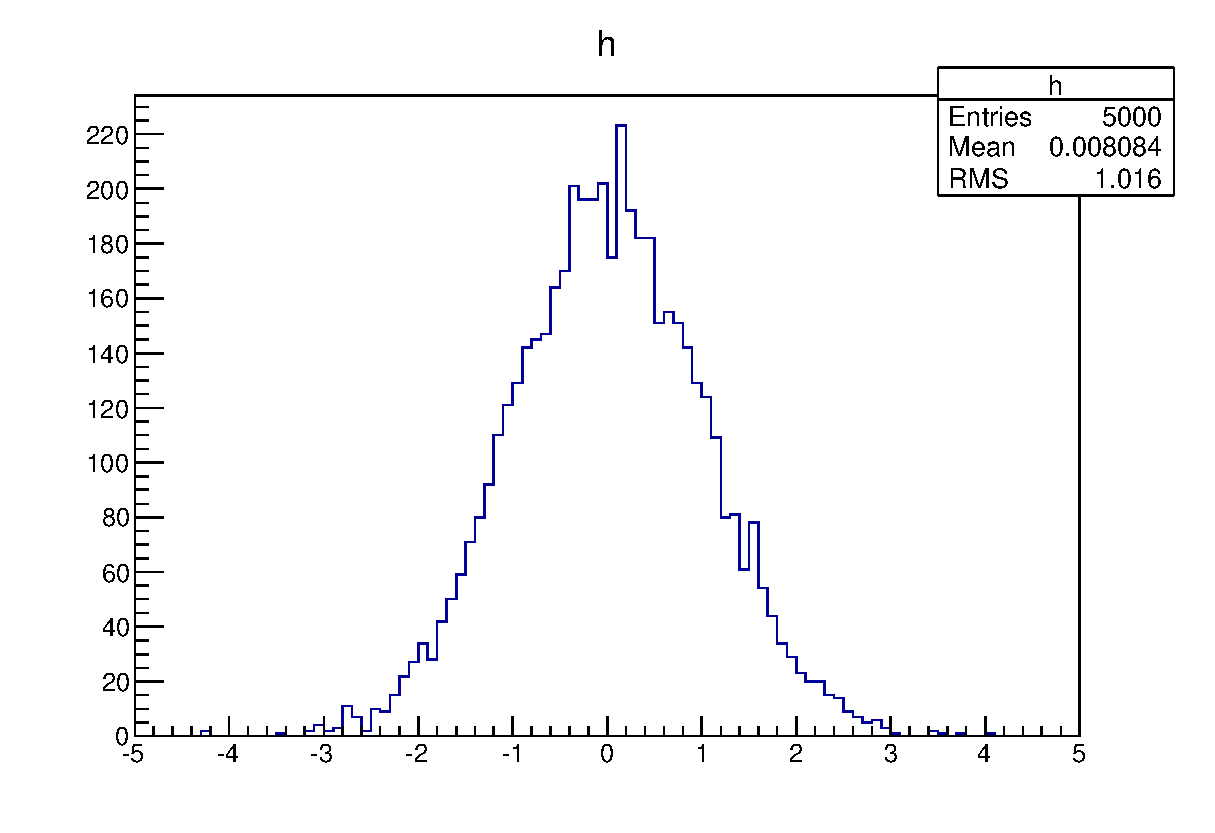
\includegraphics[width = 100mm]{./picture/hist1canvas1.eps}
  \end{center}
  \caption{ヒストグラムの図}
  \label{Fig:hist1canvas1}
 \end{figure}

  \subsection{練習}

  \begin{enumerate}
   \item ヒストグラムを統計誤差付きで評価せよ
	 \begin{description}
	  \item[ヒント] \url{http://root.cern.ch/root/html/TH1.html#TH1:Draw}
	  \item[ヒント] \url{http://root.cern.ch/root/html/THistPainter.html#HP01a}
	  \item[ヒント] \url{http://root.cern.ch/root/html/THistPainter.html#HP01b}
	 \end{description}
   \item ヒストグラムの最大値を取得せよ。
	 \begin{description}
	  \item[ヒント] \url{http://root.cern.ch/root/html/TH1.html#TH1:GetMaximum}
	 \end{description}
   \item ヒストグラムの最大値が納められたbinのbin番号を取得せよ。
	 \begin{description}
	  \item[ヒント] \url{http://root.cern.ch/root/html/TH1.html#TH1:GetMaximumBin}
	 \end{description}
   \item ヒストグラムの最大値が納められたbinのエラーの値を取得せよ。
	 \begin{description}
	  \item[ヒント] \url{http://root.cern.ch/root/html/TH1.html#TH1:GetBinError}
	 \end{description}
   \item GUIを用いてグリッドを描け。最終的に図\ref{Fig:hist1canvas2}のように描け。
	 \begin{description}
	  \item[ヒント] GUIでは<View>から<Editor>を選択する。
		     するとキャンバスの左側に様々な編集ツールが表示される。
		     \begin{figure}[htbp]
		      \begin{center}
		       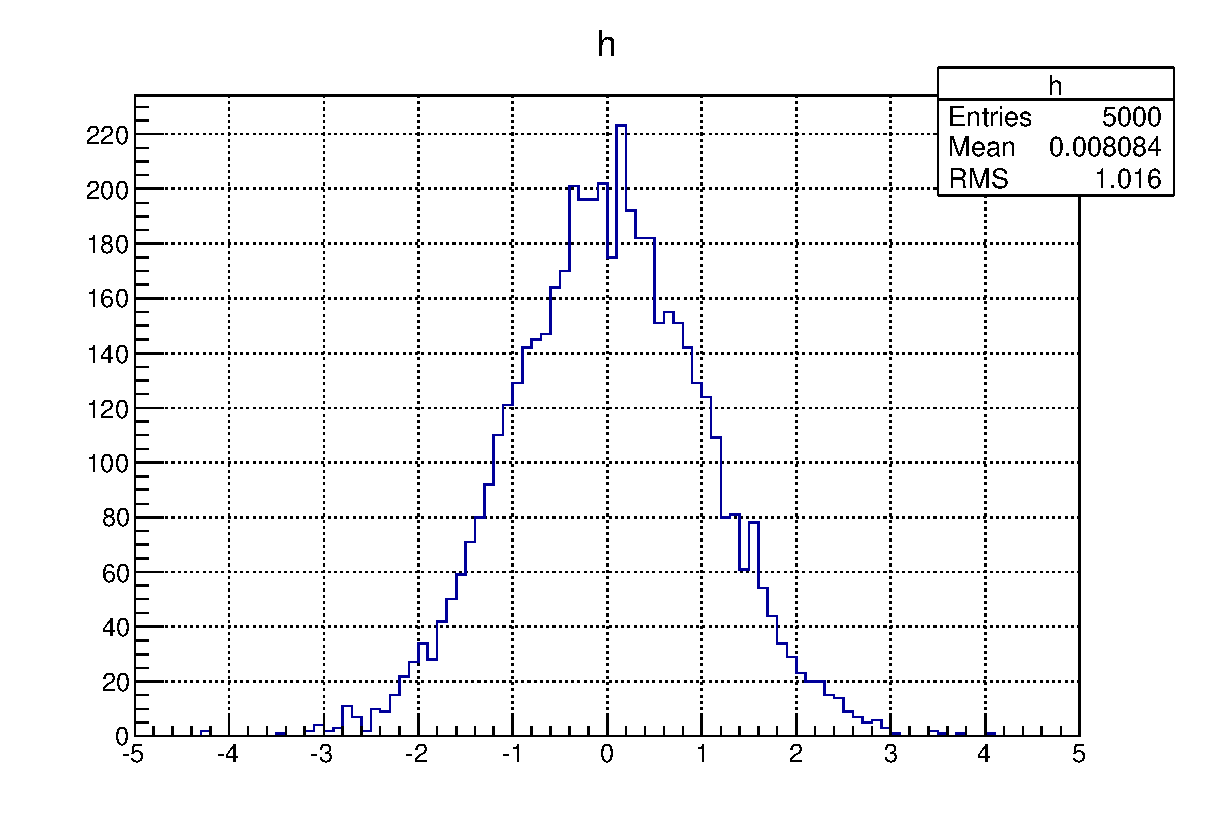
\includegraphics[width = 100mm]{./picture/hist1canvas2.eps}
		      \end{center}
		      \caption{グリッドを描いたヒストグラム}
		      \label{Fig:hist1canvas2}
		     \end{figure}
	 \end{description}
   \item \ROOT で\verb|h->Draw();|を行ったとき、 \\
	 \verb|Info in <TCanvas::MakeDefCanvas>: created default TCanvas with name c1| \\
	 というメッセージが出ただろう。文字どおり、c1というキャンバスが作られ、そこにhが描画されている。
	 c1を"c1.eps"として保存せよ。
	 \begin{description}
	  \item[ヒント] \ROOT のキャンバスなどは全て\verb|TObject|からの派生である。\\
		     \url{http://root.cern.ch/root/html/TObject.html#TObject:SaveAs}
	 \end{description}

  \end{enumerate}

  \subsection{解答例}
  \begin{enumerate}
   \item ヒストグラムを統計誤差付きで評価せよ
	 \begin{itembox}{\texttt{hist1sol1.cpp}}
\begin{verbatim}
	...
	TH1D *hist1sol1(){
	  ...
	  h->Draw("E");
	  ...
	}
\end{verbatim}
	 \end{itembox}

   \item ヒストグラムの最大値を取得せよ。
\begin{verbatim}
	root [0] .L hist1.cpp+
	root [1] hist1()
	Start!!
	Info in <TCanvas::MakeDefCanvas>:  created default TCanvas with name c1
	(class TH1D*)0x7f97b4b7bda0
	root [2] h->GetMaximum()
	(const Double_t)2.23000000000000000e+02
\end{verbatim}
   \item ヒストグラムの最大値が納められたbinのbin番号を取得せよ。
\begin{verbatim}
	root [3] h->GetMaximumBin()
	(const Int_t)52
\end{verbatim}
   \item ヒストグラムの最大値が納められたbinのエラーの値を取得せよ。
\begin{verbatim}
	root [4] int maxbinnum = h->GetMaximumBin()
	root [5] h->GetBinError(maxbinnum)
	(const Double_t)1.49331845230680784e+01
\end{verbatim}
   \item GUIを用いてグリッドを描け。最終的に図\ref{Fig:hist1canvas2}のように描け。

   \item c1を"c1.eps"として保存せよ。
\begin{verbatim}
	root [6] c1->SaveAs("c1.eps")
	Info in <TCanvas::Print>: eps file c1.eps has been created
\end{verbatim}
  \end{enumerate}
  
\clearpage
%%%%%%%%%%%%%%%%%%%%%%%%%%%%%%%%%%%%%%%%%%%%%%%%%%%%%%%%%%%%%%%%%%%%%%%%%%%%%%%%%
%%        %%%        %%%        %%%        %%%        %%%         %%%  %%%%  %%%
%%  %%%%%%%%%  %%%%%%%%%  %%%%%%%%%%%%  %%%%%%%%%  %%%%%%  %%%%%  %%%    %%  %%%
%%        %%%        %%%  %%%%%%%%%%%%  %%%%%%%%%  %%%%%%  %%%%%  %%%  %  %  %%%
%%%%%%%%  %%%  %%%%%%%%%  %%%%%%%%%%%%  %%%%%%%%%  %%%%%%  %%%%%  %%%  %%    %%%
%%        %%%        %%%        %%%%%%  %%%%%%        %%%         %%%  %%%   %%%
%%%%%%%%%%%%%%%%%%%%%%%%%%%%%%%%%%%%%%%%%%%%%%%%%%%%%%%%%%%%%%%%%%%%%%%%%%%%%%%%%
 \section{\texttt{TRandom}と\texttt{TCanvas}}

 乱数とキャンバスの操作に出会う。

 \begin{itembox}{\texttt{canran.cpp}}
\begin{verbatim}
	#include "TCanvas.h"
	#include "TH1.h"
	#include "TRandom3.h"
	#include "TStyle.h"
	TCanvas *canran(){
	  TCanvas *c1 = new TCanvas("c1","c1",600,600) ;
	  TRandom3 *r = new TRandom3();
	  TH1D *h = new TH1D("h","h-title;x;y",100,-5,5) ;
	  for(int i = 0 ; i<100000 ; i++){
	    h->Fill(r->Uniform(-3.,3.)) ;
	  }
	  h->Draw("HE") ;
	  c1->SaveAs("c1.eps") ;
	  return c1 ;
	}
\end{verbatim}
 \end{itembox}


 \begin{figure}[htbp]
  \begin{center}
   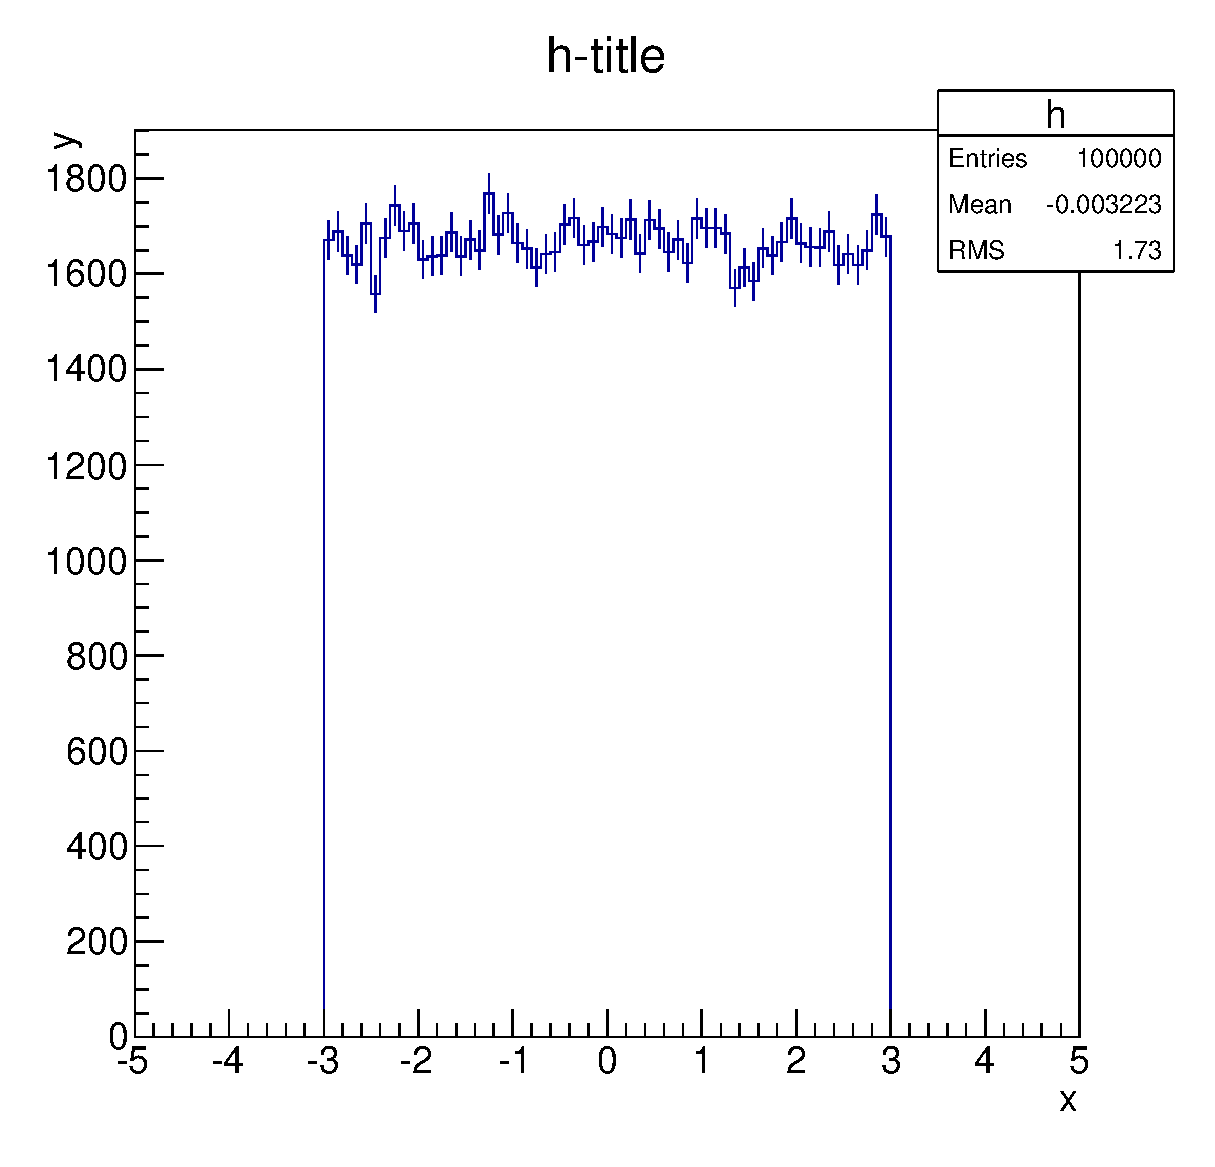
\includegraphics[width = 90mm] {./picture/canrancanvas1.eps}
  \end{center}
  \caption{\texttt{canran.cpp}の実行結果}
  \label{Fig:canrancanvas1}
 \end{figure}


  \subsection{練習}

  \begin{enumerate}

   \item プログラムの各行を説明せよ。
	 \begin{description}
	  \item[ヒント] メルセンヌツイスタとはメルセンヌ数という数の特徴を用いた乱数生成子のこと。
	  \item[ヒント] \url{http://root.cern.ch/root/htmldoc/TRandom.html}
	  \item[ヒント] \url{http://root.cern.ch/root/htmldoc/TRandom3.html}
	 \end{description}

   \item 今は
	 \verb|h->Fill(r->Uniform(-1.,1.)) ;|としているが、
	 \verb|h->Fill(r->Exp(1.)) ;|、
	 \verb|h->Fill(r->Gaus(1.,1.)) ;|、
	 \verb|h->Fill(r->Binomial(3,0.3)) ;|、
	 \verb|h->Fill(r->PoissonD(1)) ;|
	 などとした時の挙動を確かめよ。
	 \begin{description}
	  \item[ヒント] これを気に幾つかの基本的な確率分布について調べよ。
	  \item[ヒント] \url{http://root.cern.ch/root/htmldoc/TRandom.html#TRandom:Exp}
	  \item[ヒント] \url{http://root.cern.ch/root/htmldoc/TRandom.html#TRandom:Gaus}
	  \item[ヒント] \url{http://root.cern.ch/root/htmldoc/TRandom.html#TRandom:Binomial}
	  \item[ヒント] \url{http://root.cern.ch/root/htmldoc/TRandom.html#TRandom:Poisson}
	 \end{description}

   \item hist1を繰り返し実行した時にヒストグラムに変化があるかどうか検証せよ。
	 変化がない場合、この原因を突き止めて実行毎に違うヒストグラムが出来上がるような仕様へ変更せよ。
	 \begin{description} 
	  \item[ヒント] \url{http://root.cern.ch/root/htmldoc/TRandom.html#TRandom:TRandom}
	  \item[ヒント] \url{http://root.cern.ch/root/htmldoc/TRandom.html#TRandom:SetSeed}
	 \end{description}
  \end{enumerate}

  \subsection{解答例}

  \begin{enumerate}

   \item プログラムの各行を説明せよ。

   \item 今は
	 \verb|h->Fill(r->Uniform(-1.,1.)) ;|としているが、
	 \verb|h->Fill(r->Exp(1.)) ;|、
	 \verb|h->Fill(r->Gaus(1.,1.)) ;|、
	 \verb|h->Fill(r->Binomial(3,0.3)) ;|、
	 \verb|h->Fill(r->PoissonD(1)) ;|
	 などとした時の挙動を確かめよ。

   \item hist1を繰り返し実行した時にヒストグラムに変化があるかどうか検証せよ。
	 変化がない場合、この原因を突き止めて実行毎に違うヒストグラムが出来上がるような仕様へ変更せよ。
	 \begin{itembox}{\texttt{canransol1.cpp}}
\begin{verbatim}
	...
	TCanvas *canransol1(){
	  TCanvas *c1 = new TCanvas("c1","c1",600,600) ;
	  TRandom3 *r = new TRandom3() ;
	  r->SetSeed(unsigned (time(NULL))) ;
	  ...
	}
\end{verbatim}
	 \end{itembox}

  \end{enumerate}
 \clearpage
 %%%%%%%%%%%%%%%%%%%%%%%%%%%%%%%%%%%%%%%%%%%%%%%%%%%%%%%%%%%%%%%%%%%%%%%%%%%%%%%%%
 %%        %%%        %%%        %%%        %%%        %%%         %%%  %%%%  %%%
 %%  %%%%%%%%%  %%%%%%%%%  %%%%%%%%%%%%  %%%%%%%%%  %%%%%%  %%%%%  %%%    %%  %%%
 %%        %%%        %%%  %%%%%%%%%%%%  %%%%%%%%%  %%%%%%  %%%%%  %%%  %  %  %%%
 %%%%%%%%  %%%  %%%%%%%%%  %%%%%%%%%%%%  %%%%%%%%%  %%%%%%  %%%%%  %%%  %%    %%%
 %%        %%%        %%%        %%%%%%  %%%%%%        %%%         %%%  %%%   %%%
 %%%%%%%%%%%%%%%%%%%%%%%%%%%%%%%%%%%%%%%%%%%%%%%%%%%%%%%%%%%%%%%%%%%%%%%%%%%%%%%%%
 \section{TGraph}
 \ROOT を使ってx座標及びy座標を与えてグラフを描くことが大いに考えられる。
 \ROOT では\verb|TGraph|を使うことで実現できる。
 
 
\subsection{ファイルから読み込んでグラフ化する}
シンチレータと光電子増倍管を組み合わせた検出器を考える。
光電子増倍管からの信号にある閾値を設け、
光電子増倍管に印加する電圧を変化させて単位時間あたりにどれだけの収量が得られたかを測定した実験を考える。
この時、下記のような形式のデータファイルをきっと作ることだろう。
 \begin{itembox}{\texttt{plateaudata.plt}}
\begin{verbatim}
	# HV[V]  Counts[c/min]
1400  3
1450  1
1500  2
1550  10
1600  14
1650  20
1700  80
1750  250
1800  600
1850  900
1900  1000
1950  1050
2000  1060
2050  1090
2100  1095
2150  1100
2200  1105
2250  1108
2300  1109
2350  1105
2400  1110
2450  1120
2500  1150
2550  1240
2600  1350
2650  1505
2700  1700
\end{verbatim}
 \end{itembox}
\verb|plateaudata.plt|をプロットする方法はいくつか在る。
おそらく入り番簡単なのはgnuplot(\url{http://www.gnuplot.info})を用いる方法である。
gnuplotでこのテキストを図に起こす方法は下記の通り。
\begin{verbatim}
$ gnuplot
gnuplot> plot "plateaudata.plt"
\end{verbatim}

実行結果は図\ref{Fig:plateaugnuplot}のようである。

 \begin{figure}[htbp]
  \begin{minipage}{0.47\hsize}
   \begin{center}
    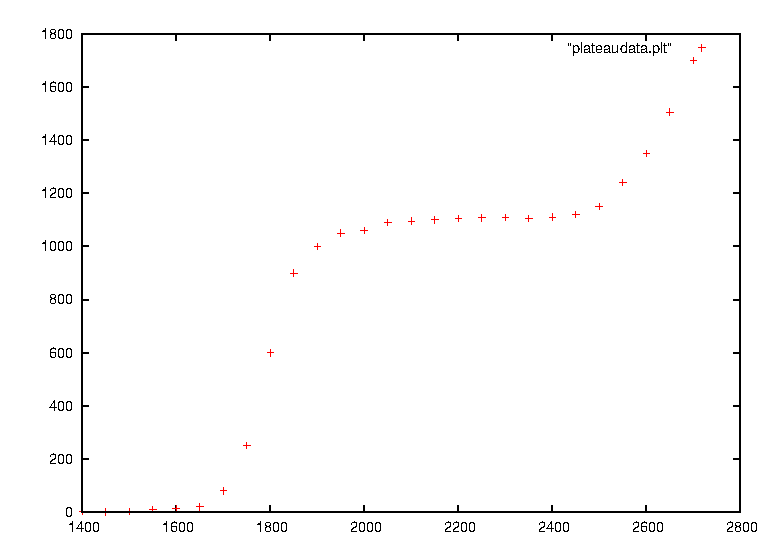
\includegraphics[width = 75mm]{./picture/plateaugnuplot.eps}
   \end{center}
   \caption{\texttt{plateaudata.plt}をgnuplotを用いて描いた時の様子。}
   \label{Fig:plateaugnuplot}
  \end{minipage}
  \begin{minipage}{0.53\hsize}
   \begin{center}
    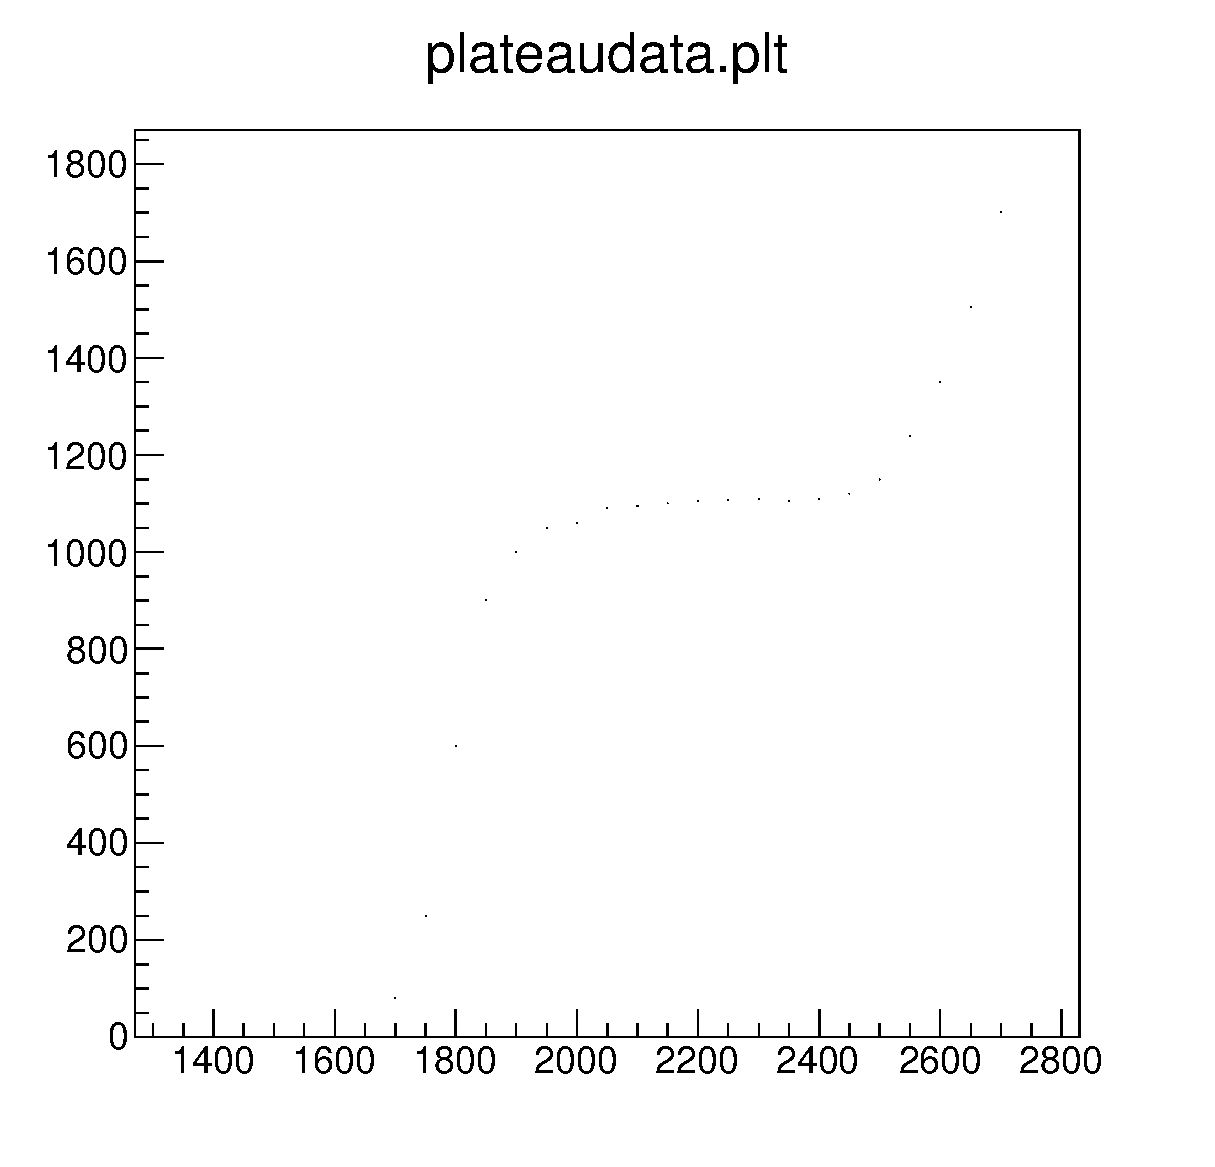
\includegraphics[width = 75mm]{./picture/plateaucanvas1.eps}
   \end{center}
   \caption{\texttt{plateaudata.plt}を\texttt{plateauplot.cpp}を用いて描いた時の様子。}
   \label{Fig:plateaucanvas1}
  \end{minipage}
 \end{figure}
 
 これを\ROOT で行う最低限のサンプルプログラムを示す。
  \begin{itembox}{\texttt{plateauplot.cpp}}
\begin{verbatim}
#include "TGraph.h"
#include "TCanvas.h"

TCanvas *plateauplot(){
  TCanvas *c1 = new TCanvas("c1", "c1", 600, 600) ;
  TGraph *f = new TGraph("plateaudata.plt", "%lf %lf") ;
  f->Draw("AP") ;
  return c1 ;
}
\end{verbatim}
  \end{itembox}
  この実行結果が図\ref{Fig:plateaucanvas1}である。
  
  
   \subsubsection{練習}
   
\begin{enumerate}
 \item プログラムの各行を理解せよ。
   \begin{description}
    \item[ヒント] \url{http://root.cern.ch/root/html/TGraph.html}
    \item[ヒント] \url{http://root.cern.ch/root/html/TGraph.html#TGraph:TGraph@10}
    \item[ヒント] \url{http://root.cern.ch/root/html/TGraph.html#TGraph:Draw}
    \item[ヒント] \url{http://root.cern.ch/root/html/TGraphPainter.html}
   \end{description}
       
 \item 引数をデータファイル名にするように変更せよ。
 \item 図\ref{Fig:plateaucanvas1}を見てわかるように、
       デフォルトではマーカーのサイズが小さい。
       マーカーサイズを調整したり、
       軸のタイトルを変更するなどしておしゃれせよ。
   \begin{description}
    \item[ヒント] \url{http://root.cern.ch/root/html/TAttMarker.html#TAttMarker:SetMarkerStyle}
    \item[ヒント] \url{http://root.cern.ch/root/html/TAttMarker.html#TAttMarker:SetMarkerSize}
    \item[ヒント] \url{http://root.cern.ch/root/html/TAttMarker.html#TAttMarker:SetMarkerColor}
    \item[ヒント] \url{http://root.cern.ch/root/html/TAttPad.html#TAttPad:SetLeftMargin}
   \end{description}
\end{enumerate}
   
   
   \subsubsection{解答例}

\begin{enumerate}
 \item プログラムの各行を理解せよ。
 \item 引数をデータファイル名にするように変更せよ。
 \item 図\ref{Fig:plateaucanvas1}を見てわかるように、
       デフォルトではマーカーのサイズが小さい。
       マーカーサイズを調整したり、
       軸のタイトルを変更するなどしておしゃれせよ。
         \begin{itembox}{\texttt{plateauplotsol1.cpp}}
\begin{verbatim}
...
TCanvas *plateauplotsol1(char *datafilename)){
  TCanvas *c1 = new TCanvas("c1", "c1", 600, 600) ;
  c1->SetGrid(1,1) ;
  c1->SetLogy() ;
  c1->SetLeftMargin(0.14) ;
  TGraph *f = new TGraph(datafilename, "%lf %lf") ;
  f->SetMarkerStyle(20) ;
  f->SetMarkerSize(1.1) ;
  f->SetMarkerColor(kRed) ;
  f->SetTitle("Plateau Curve") ;
  f->GetXaxis()->SetTitle("Voltage[V]") ;
  f->GetYaxis()->SetTitle("Counts[c/min]") ;
  f->GetYaxis()->SetTitleOffset(1.4) ;
  f->Draw("AP") ;
  return c1 ;
}
\end{verbatim}
  \end{itembox}
\begin{figure}[htbp]
   \begin{center}
    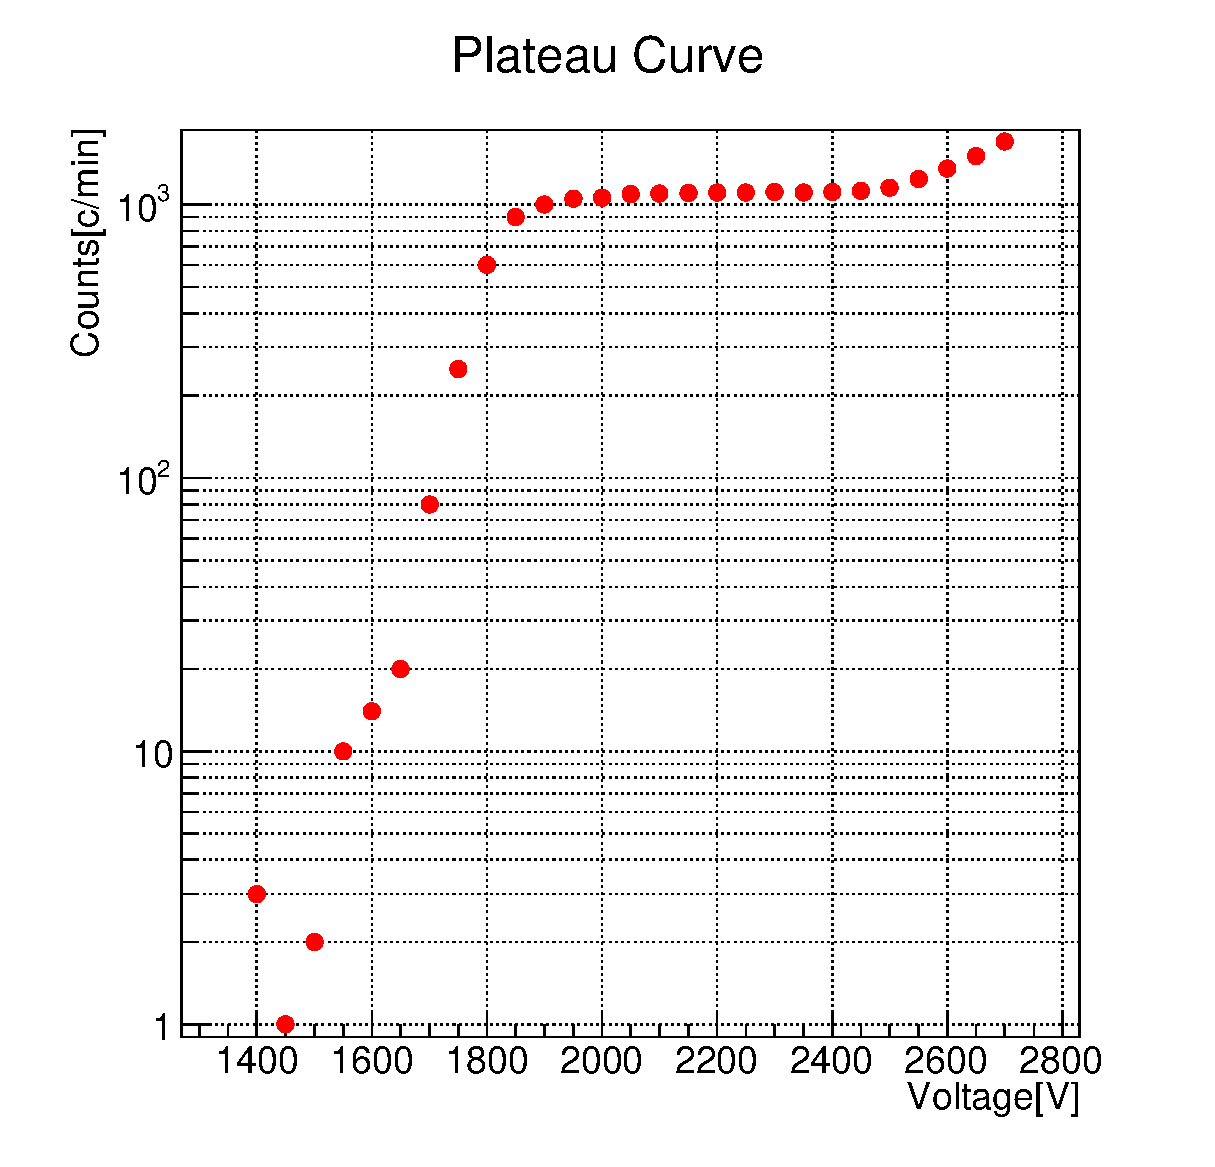
\includegraphics[width = 75mm]{./picture/plateaucanvas2.eps}
   \end{center}
   \caption{\texttt{plateauplotsol1.cpp}の実行結果。}
   \label{Fig:plateaucanvas2}
\end{figure}
\end{enumerate}



 
 
\subsection{ランダムウォーク}
 \begin{itembox}{\texttt{randomwalk.cpp}}
\begin{verbatim}
#include "TRandom3.h"
#include "TCanvas.h"
#include "TGraph.h"

TCanvas *randomwalk(){
  const int imax = 100 ;
  double x[imax] = {0.} ;
  double y[imax] = {0.} ;

  TRandom3 RandomGenerator(unsigned(time(NULL))) ;
  TCanvas *c1 = new TCanvas("c1", "c1", 600,600) ;
  c1->SetGrid(1,1) ;  
  for(int i = 1 ; i < imax ;i++){
    x[i] = RandomGenerator.Uniform(-1., 1.) + x[i-1] ; // 前の位置から[-1,1]だけx座標を移動
    y[i] = RandomGenerator.Uniform(-1., 1.) + y[i-1] ; // 前の位置から[-1,1]だけy座標を移動
  }
  TGraph  *f  = new TGraph(imax, x, y) ;
  f->SetLineStyle(1) ;
  f->SetLineWidth(2) ;
  f->SetLineColor(kRed) ;
  f->SetMarkerStyle(20) ;
  f->SetMarkerSize(1.1) ;
  f->SetMarkerColor(kBlue) ;

  f->Draw("APL") ;
  return c1 ;
}
\end{verbatim}
  \end{itembox}
 \begin{figure}[htbp]
  \begin{center}
   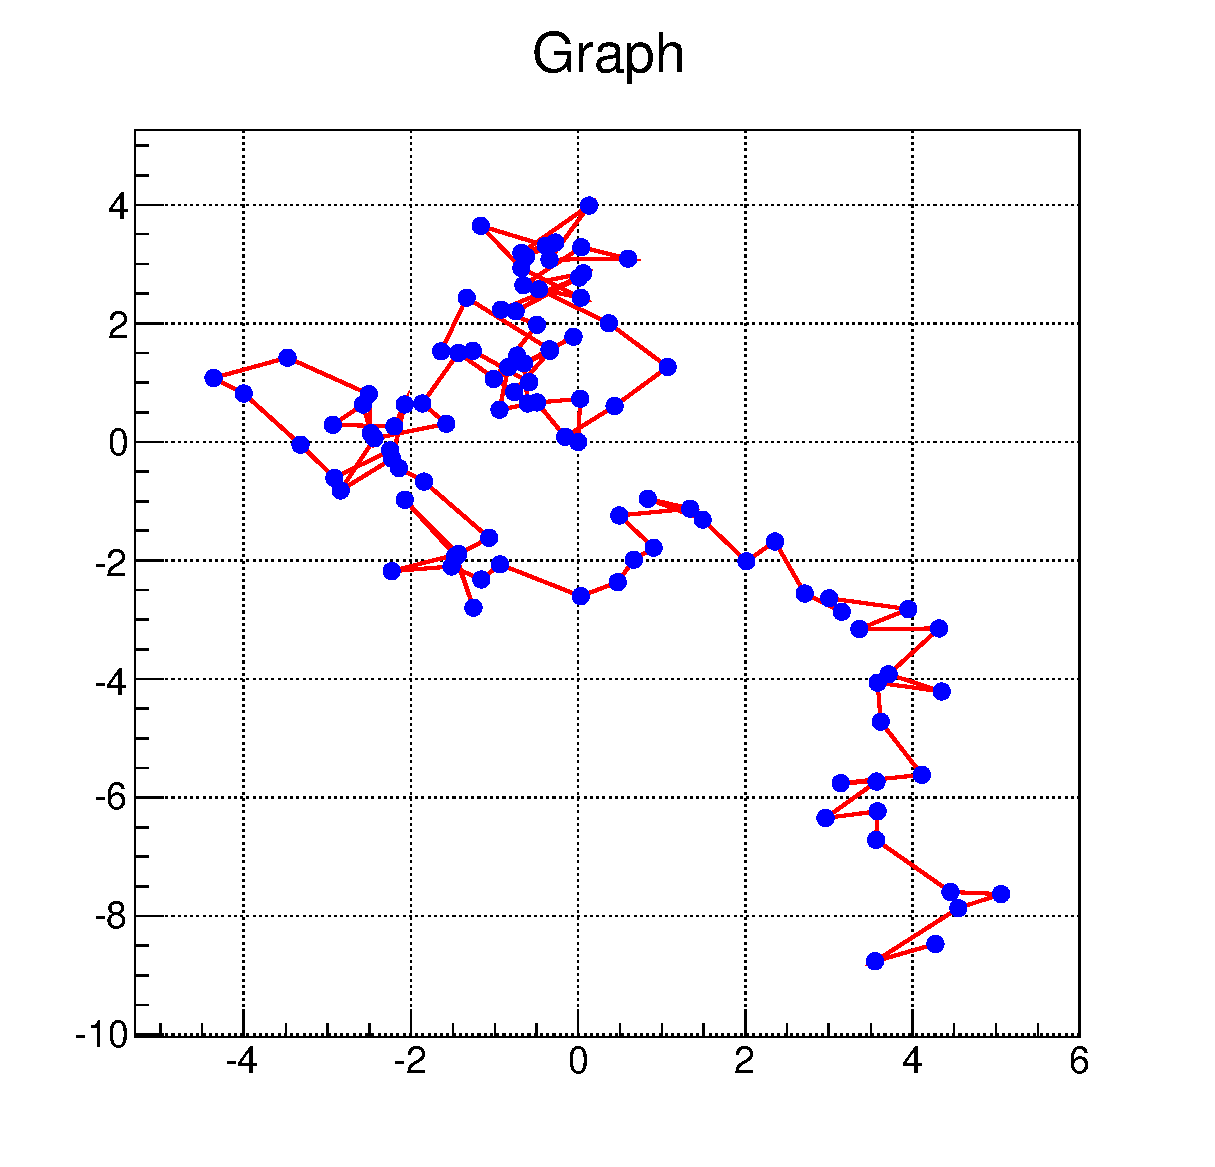
\includegraphics[width = 90mm]{./picture/randomwalkcanvas1.eps}
  \end{center}
  \caption{\texttt{randomwalk.cpp}の実行結果}
  \label{Fig:randomwalkcanvas1}
 \end{figure}

\subsubsection{練習}
\begin{enumerate}
 \item プログラムの各行を説明せよ
   \begin{description}
    \item[ヒント] \url{http://root.cern.ch/root/html/TGraph.html}
    \item[ヒント] \url{http://root.cern.ch/root/html/TGraph.html#TGraph:TGraph@2}
   \end{description}
 \item 今はx,yそれぞれの変化は[-1,1]で与えているが、
       現在位置から半径1の円周上が新しい点になるようにプログラムを変更せよ。
       これはTGraphの練習というよりも乱数の練習である。
   \begin{description}
    \item[ヒント] \url{http://root.cern.ch/root/htmldoc/TRandom.html#TRandom:Circle}
   \end{description}
       
\end{enumerate}

\subsubsection{解答例}

\begin{enumerate}
 \item プログラムの各行を説明せよ
 \item 今はx,yそれぞれの変化は[-1,1]で与えているが、
       現在位置から半径1の円周上が新しい点になるようにプログラムを変更せよ。
       \begin{itembox}{\texttt{randomwalksol1.cpp}}
\begin{verbatim}
...
TCanvas *randomwalksol1(){
  const int imax = 100 ;
  double x[imax] = {0.} ;
  double y[imax] = {0.} ;
  double deltax ;
  double deltay ;
  double radius = 1.0 ;
...
  for(int i = 1 ; i < imax ;i++){
    RandomGenerator.Circle(deltax, deltay, radius) ; // 半径radiusの円周上に一様に乱数を生成する。
    x[i] = deltax + x[i-1]; // 前の座標からdeltaxだけ移動する
    y[i] = deltay + y[i-1]; // 前の座標からdeltayだけ移動する
  }
  TGraph  *f  = new TGraph(imax, x, y) ;
...
\end{verbatim}
       \end{itembox}
念のため、
実行方法は次の通り。
\begin{verbatim}
$ root
root[0] .L plateauplotsol1.cpp+
root[1] plateauplotsol1("plateaudata.plt")
\end{verbatim}
\end{enumerate}

\clearpage
%%%%%%%%%%%%%%%%%%%%%%%%%%%%%%%%%%%%%%%%%%%%%%%%%%%%%%%%%%%%%%%%%%%%%%%%%%%%%%%%%
%%        %%%        %%%        %%%        %%%        %%%         %%%  %%%%  %%%
%%  %%%%%%%%%  %%%%%%%%%  %%%%%%%%%%%%  %%%%%%%%%  %%%%%%  %%%%%  %%%    %%  %%%
%%        %%%        %%%  %%%%%%%%%%%%  %%%%%%%%%  %%%%%%  %%%%%  %%%  %  %  %%%
%%%%%%%%  %%%  %%%%%%%%%  %%%%%%%%%%%%  %%%%%%%%%  %%%%%%  %%%%%  %%%  %%    %%%
%%        %%%        %%%        %%%%%%  %%%%%%        %%%         %%%  %%%   %%%
%%%%%%%%%%%%%%%%%%%%%%%%%%%%%%%%%%%%%%%%%%%%%%%%%%%%%%%%%%%%%%%%%%%%%%%%%%%%%%%%%
 \section{任意の関数に従うヒストグラムを描く}
 自分で定義した関数に従って乱数を生成してヒストグラムを描こう。
 \begin{itembox}{\texttt{ranfun.cpp}}
\begin{verbatim}
	#include "TCanvas.h"
	#include "TF1.h"
	#include "TH1.h"
	#include "TMath.h"
	TH1D *ranfun(){
	  double range_min = 0. ; // 0 [ns]
	  double range_max = 8000.e-9 ;// 8000 [ns]
	  double tau       = 2.2e-6 ; // it means lifetime
	  double bgd = 0.5 ; // Background
	  int nbin = 100 ; // histgram bin num
	  int imax = 100000 ; // event

	  TCanvas *c1 = new TCanvas("c1","c1",600,600) ;
	  c1->SetGrid(1,1) ; // Canvas c1 にグリッドを描く
	  c1->SetLogy(1) ;  // Canvas c1 の縦軸をlogで

	  TF1 *f = new TF1("f","TMath::Exp(-x/[0])+[1]", range_min, range_max) ;
	  f->SetParameter(0, tau) ;
	  f->SetParameter(1, bgd) ;
	  //  f->SetParameters(tau,bgd) ; // <--上の二行はこの一行と等価

	  TH1D *h = new TH1D("h","Decay curve (Muon);TDC [s] ; Counts ", nbin, range_min, range_max) ;
	  for(int i=0; i < imax; i++){
	    h->Fill(f->GetRandom()) ;
	  }
	  h->Draw("HE") ;

	  /********************************************************************************\
	  * Decay Curve Fitting
	  \********************************************************************************/
	  /* If you want to use fit, then please uncomment
	  gStyle->SetOptFit(1101) ;
	  TF1 *muon = new TF1("muon","[0]*TMath::Exp(-x/[1])+[2]") ;
	  muon->SetParameters(2e+3, 2e-6, 1e+2) ;
	  muon->SetLineColor(kBlue) ;
	  muon->SetLineWidth(4) ;
	  h->Fit(muon) ;
	  */
	  return h ;
	}
\end{verbatim}
 \end{itembox}

  \subsection{練習}
  \begin{enumerate}
   \item プログラムの各行の役割を理解せよ。
	 \begin{description}
	  \item[ヒント] \url{http://root.cern.ch/root/html/TF1.html#TF1:GetRandom}
	 \end{description}

   \item 図\ref{Fig:ranfunsol1canvas1}のようなおしゃれをしたヒストグラムを描け。
	 \begin{figure}[htbp]
	  \begin{center}
	   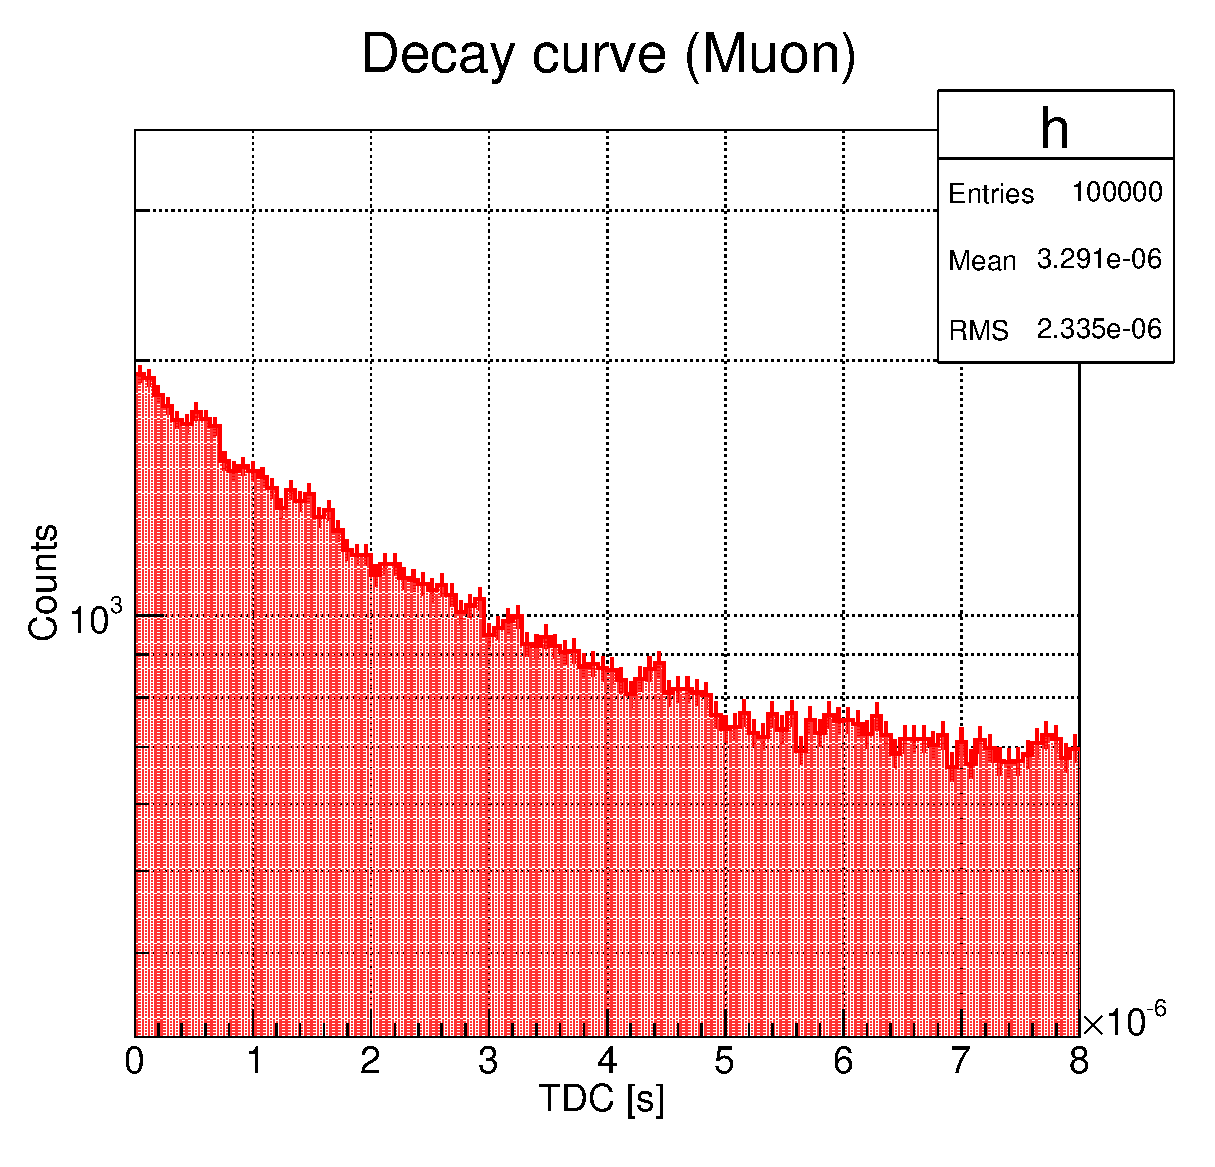
\includegraphics[width = 90mm]{./picture/ranfunsol1canvas1.eps}
	  \end{center}
	  \caption{各種の設定をいじったヒストグラム}
	  \label{Fig:ranfunsol1canvas1}
	 \end{figure}
	 \begin{description}
	  \item[ヒント] \url{http://root.cern.ch/root/html/TH1.html#TH1:GetXaxis}
	  \item[ヒント] \url{http://root.cern.ch/root/htmldoc/TAxis.html#TAxis:CenterTitle}
	  \item[ヒント] \url{http://root.cern.ch/root/html/TH1.html#TH1:SetTitleOffset}
	  \item[ヒント] \url{http://root.cern.ch/root/html/TAttFill.html#TAttFill:SetFillColor}
	  \item[ヒント] \url{http://root.cern.ch/root/html/TAttFill.html#TAttFill:SetFillStyle}
	 \end{description}

   \item \verb|ranfun.cpp|の下部\verb|Decay Curve Fitting|以下のコメントアウトされている箇所\verb|/* ... */|をアンコメントして実行してみよ。
	 \begin{description}
	  \item[ヒント] この状態で\verb|ranfun.cpp|をコンパイルオプション付きでロードしたらエラーメッセージが出るだろう。
		     何を\verb|include|すべきかはコンパイラが認識し兼ねている単語と'ライブラリ'などの言葉と一緒に検索せよ。
		     それが\ROOT に関連しているものであれば各\verb|class|を説明しているページの右上に何を\verb|include|すべきかが書いてある。\\
		     \url{http://root.cern.ch/root/html/TStyle.html}
	 \end{description}
	 \begin{figure}[htbp]
	  \begin{center}
	   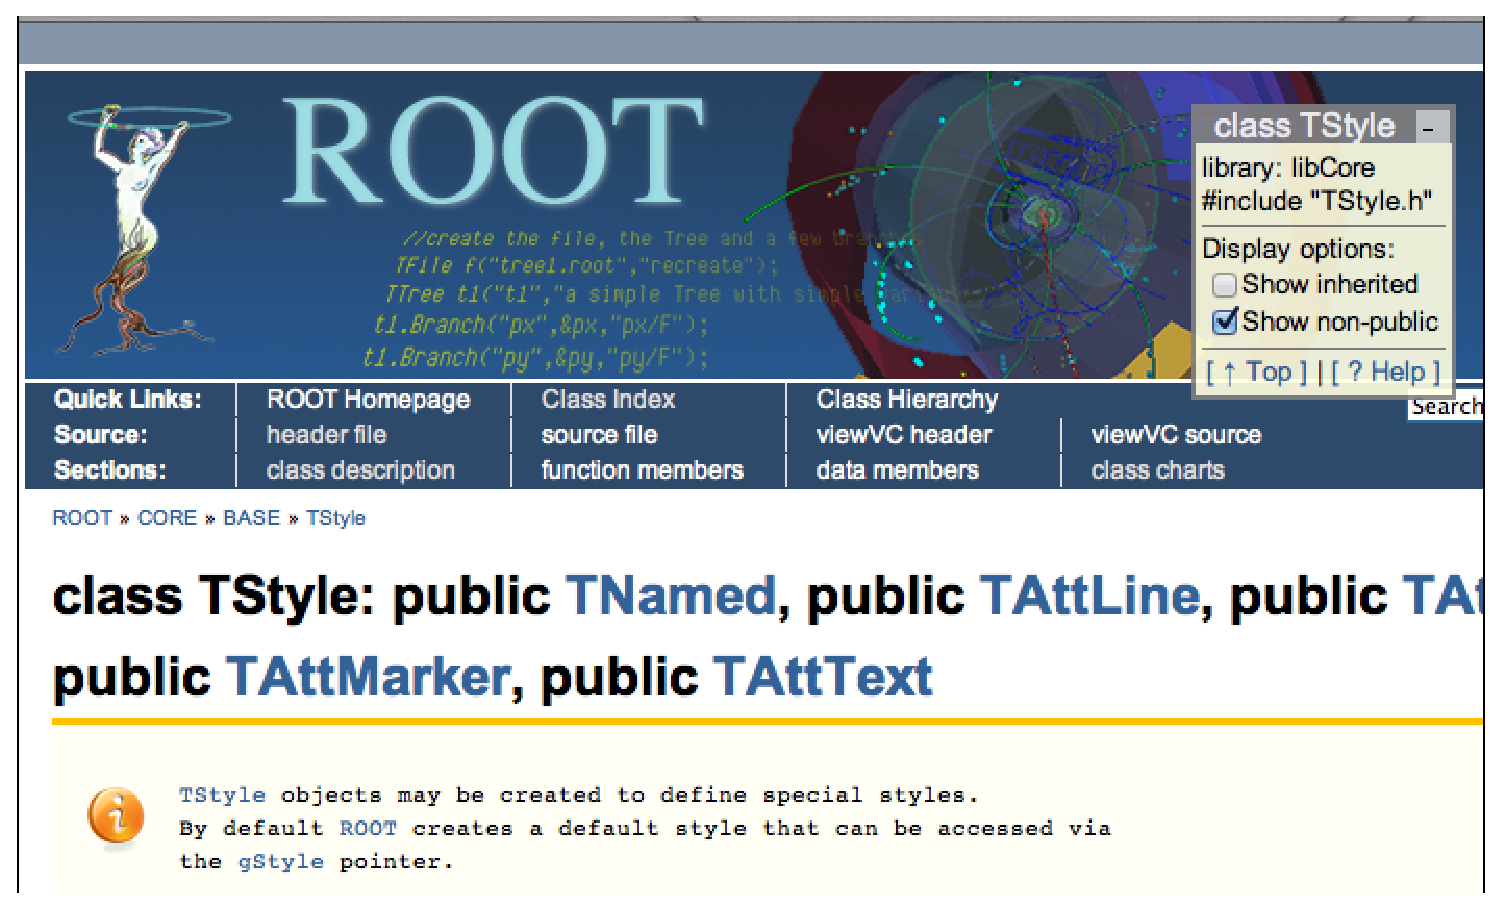
\includegraphics[width = 90mm]{./picture/classinclude.eps}
	  \end{center}
	  \label{Fig:classinclude}
	 \end{figure}
   \item フィッティングの情報が誤差付きで描かれるように変更せよ。
	 \begin{description}
	  \item[ヒント]  \url{http://root.cern.ch/root/html/TStyle.html#TStyle:SetOptFit}
	 \end{description}
  \end{enumerate}

  \subsection{解答例}

  \begin{enumerate}
   \item プログラムの各行の役割を理解せよ。

   \item 図\ref{Fig:ranfunsol1canvas1}のようなおしゃれをしたヒストグラムを描け。
	 \begin{itembox}{\texttt{ranfunsol1.cpp}}
\begin{verbatim}
	...
	TH1D  *ranfunsol1(){ 
	  ...
	  h->GetXaxis()->CenterTitle() ;
	  h->GetYaxis()->CenterTitle() ;
	  h->GetYaxis()->SetTitleOffset(1.4) ;
	  h->SetFillStyle(3002) ;
	  h->SetFillColor(kRed-4) ;
	  h->SetLineColor(kRed) ;
	  h->SetLineWidth(2) ;
	  ...
	}
\end{verbatim}
	 \end{itembox}

   \item \verb|ranfun.cpp|の下部\verb|Decay Curve Fitting|以下のコメントアウトされている箇所\verb|/* ... */|をアンコメントして実行してみよ。

   \item フィッティングの情報が誤差付きで描かれるように変更せよ。
	 \begin{itembox}{\texttt{ranfunsol2.cpp}}
\begin{verbatim}
	...
	TH1D  *ranfunsol2(){ 
	  ...
	  // If you want to use fit, then please uncomment
	  gStyle->SetOptFit(1111) ;
	  TF1 *muon = new TF1("muon","[0]*TMath::Exp(-x/[1])+[2]") ;
	  muon->SetParameters(2e+3, 2e-6, 1e+2) ;
	  muon->SetLineColor(kBlue) ;
	  muon->SetLineWidth(4) ;
	  h->Fit(muon) ;
	  ...
	}
\end{verbatim}
	 \end{itembox}
	 \begin{figure}[htbp]
	  \begin{center}
	   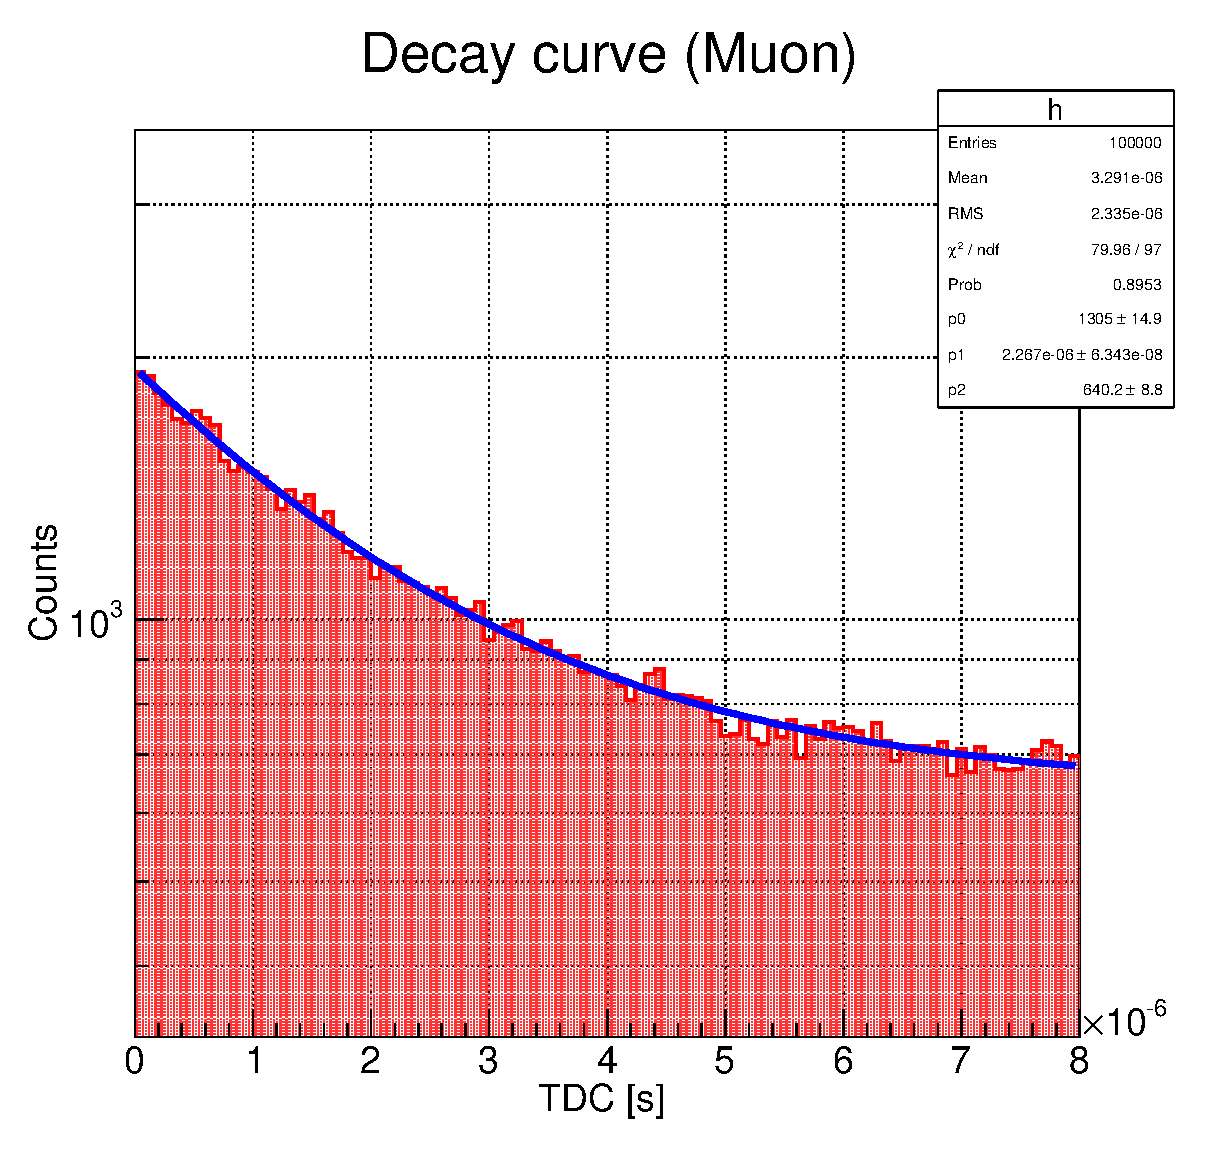
\includegraphics[width = 90mm]{./picture/ranfunsol2canvas1.eps}
	  \end{center}
	  \caption{\texttt{ranfunsol2.cpp}の実行結果}
	  \label{Fig:ranfunsol2canvas1}
	 \end{figure}

  \end{enumerate}

  \clearpage
  %%%%%%%%%%%%%%%%%%%%%%%%%%%%%%%%%%%%%%%%%%%%%%%%%%%%%%%%%%%%%%%%%%%%%%%%%%%%%%%%%
  %%        %%%        %%%        %%%        %%%        %%%         %%%  %%%%  %%%
  %%  %%%%%%%%%  %%%%%%%%%  %%%%%%%%%%%%  %%%%%%%%%  %%%%%%  %%%%%  %%%    %%  %%%
  %%        %%%        %%%  %%%%%%%%%%%%  %%%%%%%%%  %%%%%%  %%%%%  %%%  %  %  %%%
  %%%%%%%%  %%%  %%%%%%%%%  %%%%%%%%%%%%  %%%%%%%%%  %%%%%%  %%%%%  %%%  %%    %%%
  %%        %%%        %%%        %%%%%%  %%%%%%        %%%         %%%  %%%   %%%
  %%%%%%%%%%%%%%%%%%%%%%%%%%%%%%%%%%%%%%%%%%%%%%%%%%%%%%%%%%%%%%%%%%%%%%%%%%%%%%%%%
 \section{Fileへの出力}

 \begin{itembox}{\texttt{fileout.cpp}}
\begin{verbatim}
	#include "TCanvas.h"
	#include "TH1.h"
	#include "TMath.h"
	#include "TRandom3.h"
	#include <fstream>
	#include <iostream>
	TCanvas *fileout(){
	std::ofstream outputfile; // file の出力先
	outputfile.open("output.plt" );// file を開く

	TRandom3 Random(unsigned(time(NULL)));

	TCanvas *c1 = new TCanvas("c1","c1") ;

	int imax = 100000; // event 数の最大値
	double start ; // start の時刻を擬似的に与える。 
	double stop  ; // stop の時刻を擬似的に与える。 
	double tdc   ; // TDC でのカウント数を擬似的に与える。
	double life = 2.2e-6 ; // Muon の平均寿命を入力する。

	TH1D *h1 = new TH1D("h1","h1",200,0,8000e-9) ; // [s]
	for(int i = 0; i < imax; i++){
	start = Random.Uniform(0., 1.e-9) ; // start の時刻を擬似的に与える。
	stop = Random.Exp(life) ; // 指数関数に従った乱数だけ立った時刻を stop とする
	stop += start ; // start してから 指数関数に従った乱数だけ立った時刻を stop とする
	tdc = stop - start ; // このプログラムだけを見るとこの処理は余分な処理だが、TDC の理の為
	std::cout << tdc << " [s] :: " << start << "" << stop << std::endl;
	// output という出力先に start と stop をスペース区切りで出力する
	outputfile << start << " " << stop << " " << endl ;
	h1->Fill(tdc) ; // ヒストグラムに詰める
	}
	h1->Draw("H") ; // 確認用にヒストグラムを出力する。
	outputfile.close(); // ファイルを閉じる return c1 ;
	}

\end{verbatim}
 \end{itembox}

 \begin{itembox}{\texttt{output.plt}}
\begin{verbatim}
	4.8318e-10 1.59013e-06 
	8.88674e-11 2.45466e-06 
	8.04413e-10 1.65805e-06 
	...
\end{verbatim}
 \end{itembox}


 \begin{enumerate}
  \item プログラムの各行を理解せよ
	\begin{description}
	 \item[ヒント] \verb|<fstream>| なるものを\verb|include|している。これはファイル操作の時に今回使用するライブラリである。(今回は使用していないが、\ROOT には\verb|TFile.h|なるクラスも存在する。)
	\end{description}

  \item 出力先のファイル名を今はマクロ内に直書きしているが、出力先のファイルを output2.plt にしたい時に
\begin{verbatim}
	root[0] .L fileoutsol1.cpp+
	root[1] fileout("output2.plt") 
\end{verbatim}
	としたら、自動的に出力先がoutput2.pltに出来る仕様に変更せよ.
	\begin{description}
	 \item[ヒント]  \verb|TCanvas *fileout(){HogeHoge }|において引数の中身(\verb|()|の中身)は今まで何も書いてきませんでしたが、
		    この中には引数を入れることができます。引数をint型の数字\verb|_intnum|にしたいのであれば \\ \verb|TCanvas *fileout(int _intnum ){HogeHoge }|などとして、\verb|{}|内では\verb|_intnum|を定義された\verb|int|型数字だと扱えばいいだけである。では文字列ではどうすればよいか。

	\end{description}
 \end{enumerate}

  \subsection{解答例}
  \begin{enumerate}
   \item プログラムの各行を理解せよ

   \item  出力先のファイル名を今はマクロ内に直書きしているが、出力先のファイルを output2.plt にしたい時に
\begin{verbatim}
	root[0] .L fileoutsol1.cpp+
	root[1] fileout("output2.plt") 
\end{verbatim}
	  としたら、自動的に出力先がoutput2.pltに出来る仕様に変更せよ.

	  \begin{itembox}{\texttt{fileoutsol1.cpp}}
\begin{verbatim}
	...
	TCanvas *fileoutsol1(char *outputfilename){
	std::ofstream outputfile; // file の出力先
	outputfile.open(outputfilename );// file を開く
	...
	}
\end{verbatim}
	  \end{itembox}

\begin{verbatim}
	root[0] .L fileoutsol1.cpp+
	root[1] fileoutsol1("output2.plt") 
\end{verbatim} 

  \end{enumerate}
  \clearpage
  %%%%%%%%%%%%%%%%%%%%%%%%%%%%%%%%%%%%%%%%%%%%%%%%%%%%%%%%%%%%%%%%%%%%%%%%%%%%%%%%%
  %%        %%%        %%%        %%%        %%%        %%%         %%%  %%%%  %%%
  %%  %%%%%%%%%  %%%%%%%%%  %%%%%%%%%%%%  %%%%%%%%%  %%%%%%  %%%%%  %%%    %%  %%%
  %%        %%%        %%%  %%%%%%%%%%%%  %%%%%%%%%  %%%%%%  %%%%%  %%%  %  %  %%%
  %%%%%%%%  %%%  %%%%%%%%%  %%%%%%%%%%%%  %%%%%%%%%  %%%%%%  %%%%%  %%%  %%    %%%
  %%        %%%        %%%        %%%%%%  %%%%%%        %%%         %%%  %%%   %%%
  %%%%%%%%%%%%%%%%%%%%%%%%%%%%%%%%%%%%%%%%%%%%%%%%%%%%%%%%%%%%%%%%%%%%%%%%%%%%%%%%%
 \section{Fileからの入力}
 先程出力したファイルからデータを読み込んでヒストグラムを描くことを経験しよう。

 \begin{itembox}{\texttt{filein.cpp}}
\begin{verbatim}
	#include "TCanvas.h"
	#include "TF1.h"
	#include "TH1.h"
	#include "TMath.h"
	#include "TStyle.h"
	#include <fstream>
	TCanvas *filein(char *file_name){
	double range_min = 0. ;
	double range_max = 8000.e-9 ;// 8000 [ns]
	int nbin = 100 ;  
	double start ; // TDC start
	double stop  ; // TDC stop
	double tdc   ; // delta T

	TCanvas *c1 = new TCanvas("c1","c1",600,600) ;
	c1->SetGrid(1,1); // Canvas c1 にグリッドを描く
	c1->SetLogy(1) ;  // Canvas c1 の縦軸をlogで
	gStyle->SetOptFit(1) ;
	TH1D *h = new TH1D(file_name,"Decay curve (Muon);TDC [s] ; Counts ",
	nbin, range_min, range_max);
	ifstream fin(file_name) ;
	while(fin >> start >> stop){
	tdc = stop - start ;
	h -> Fill(tdc) ;
	}
	h->Draw("HE");

	/******************************************************************************** \
	* Decay Curve Fitting
	\********************************************************************************/
	TF1 *muon = new TF1("muon","[0]*(TMath::Exp(-x/[1])+[2])") ;
	muon->SetParameters(2e+3, 2e-6, 0.5) ;
	muon->SetLineColor(kBlue) ;
	muon->SetLineWidth(4) ;
	h->Fit(muon) ;

	return c1 ;
	}
\end{verbatim}
 \end{itembox}


 \clearpage
 %%%%%%%%%%%%%%%%%%%%%%%%%%%%%%%%%%%%%%%%%%%%%%%%%%%%%%%%%%%%%%%%%%%%%%%%%%%%%%%%%
 %%        %%%        %%%        %%%        %%%        %%%         %%%  %%%%  %%%
 %%  %%%%%%%%%  %%%%%%%%%  %%%%%%%%%%%%  %%%%%%%%%  %%%%%%  %%%%%  %%%    %%  %%%
 %%        %%%        %%%  %%%%%%%%%%%%  %%%%%%%%%  %%%%%%  %%%%%  %%%  %  %  %%%
 %%%%%%%%  %%%  %%%%%%%%%  %%%%%%%%%%%%  %%%%%%%%%  %%%%%%  %%%%%  %%%  %%    %%%
 %%        %%%        %%%        %%%%%%  %%%%%%        %%%         %%%  %%%   %%%
 %%%%%%%%%%%%%%%%%%%%%%%%%%%%%%%%%%%%%%%%%%%%%%%%%%%%%%%%%%%%%%%%%%%%%%%%%%%%%%%%%
 \section{treeに出会う}

 \ROOT には拡張子に\verb|.root|を拡張子としたファイルがある。
 (以下\verb|root|ファイルと呼ぶ。)
 ここでは\verb|root|ファイルにデータを詰める方法とその使い方を示す。
 やることは
 \begin{enumerate}
  \item startとstopの2行が書かれたデータを開く
  \item startとstop、及びその差を読んでTDCの値とする。
  \item start、stop、TDCの値をTreeというものに格納する。\\
	\url{http://root.cern.ch/drupal/content/ttree-and-its-data}
  \item Treeを\verb|root|ファイルに書き出す。
 \end{enumerate}

 \begin{itembox}{\texttt{meettree.cpp}}
\begin{verbatim}
	#include <fstream>
	#include "TFile.h"
	#include "TTree.h"

	TTree *meettree(char *datafile, char *rootfile = "output.root"){

	double start ; // TDC start
	double stop  ; // TDC stop
	double tdc   ; // delta T

	TTree *tree = new TTree("tree","tree");  //TTree作成
	//Branch準備
	tree->Branch( "start", &start, "start/D" ); // start を格納する為のブランチ
	tree->Branch( "stop" , &stop , "stop/D" );  // stop を格納する為のブランチ
	tree->Branch( "tdc"  , &tdc  , "tdc/D" );   // start とstopの時間差 を格納する為のブランチ

	ifstream fin(datafile) ;
	while(fin >> start >> stop){
	tdc = stop - start ;
	tree->Fill() ;
	}

	TFile *fout = new TFile(rootfile, "recreate");
	tree->Write(); // treeを書き込む
	fout->Close(); // file close

	return tree ;
	}
\end{verbatim}
 \end{itembox}

  \subsection{\texttt{meettree.cpp}を実行する}
\begin{verbatim}
	$ root
	root [0] .L meettree.cpp+
	root [1] meettree("output.plt","test.root")
	(class TTree*)0x7fc1d22a1b70
\end{verbatim}
すると、作業ディレクトリに\verb|test.root|というファイルが出来ている。
(出力ファイルのデフォルト名は\verb|output.root|なので、\verb|meettree|実行時に第二引数を指定しなかった場合、
出来上がる\verb|root|ファイルは\verb|output.root|である。)
これが\verb|root|ファイルである。

  \subsection{Treeを扱う}
  以降、前節で出力したファイル名が\verb|test.root|だとして話を進める。
  \verb|test.root|に収められているTreeの扱いの走りを紹介する。
\begin{verbatim}
	$ root  test.root 
	root [0] 
	Attaching file test.root as _file0...
\end{verbatim}
次に、今我々が扱えるものが何かを表示する。
\begin{verbatim}
	root[1] .ls
	TFile**		test.root
	TFile*		test.root
	KEY: TTree	tree;1	tree
\end{verbatim}
\verb|tree|というのが存在するのがわかる。
\verb|tree|の情報を表示するには、\verb|Print|を使う。
\begin{verbatim}
	root [2] tree->Print()
	******************************************************************************
	*Tree    :tree      : tree                                                   *
	*Entries :   100000 : Total =         4808328 bytes  File  Size =    2406559 *
	*        :          : Tree compression factor =   2.00                       *
	******************************************************************************
	*Br    0 :start     : start/D                                                *
	*Entries :   100000 : Total  Size=    1602694 bytes  File Size  =     801872 *
	*Baskets :       26 : Basket Size=      32000 bytes  Compression=   2.00     *
	*............................................................................*
	*Br    1 :stop      : stop/D                                                 *
	*Entries :   100000 : Total  Size=    1602664 bytes  File Size  =     801846 *
	*Baskets :       26 : Basket Size=      32000 bytes  Compression=   2.00     *
	*............................................................................*
	*Br    2 :tdc       : tdc/D                                                  *
	*Entries :   100000 : Total  Size=    1602634 bytes  File Size  =     801820 *
	*Baskets :       26 : Basket Size=      32000 bytes  Compression=   2.00     *
	*............................................................................*
\end{verbatim}
これらがtreeで扱える情報である。

  \subsection{Treeからヒストグラムを描く}
  treeに入った情報を書き出すのは簡単である。
\begin{verbatim}
	root [3] tree->Draw("start")
	Info in <TCanvas::MakeDefCanvas>:  created default TCanvas with name c1
	root [4] tree->Draw("stop")
\end{verbatim}
などとすれば、ヒストグラムが描かれる。
(このテキストの\verb|fileout.cpp|でどのような乱数で\verb|start|や\verb|stop|を与えたのかを思い出せ。)

\begin{figure}[htbp]
 \begin{minipage}{0.45\hsize}
  \begin{center}
   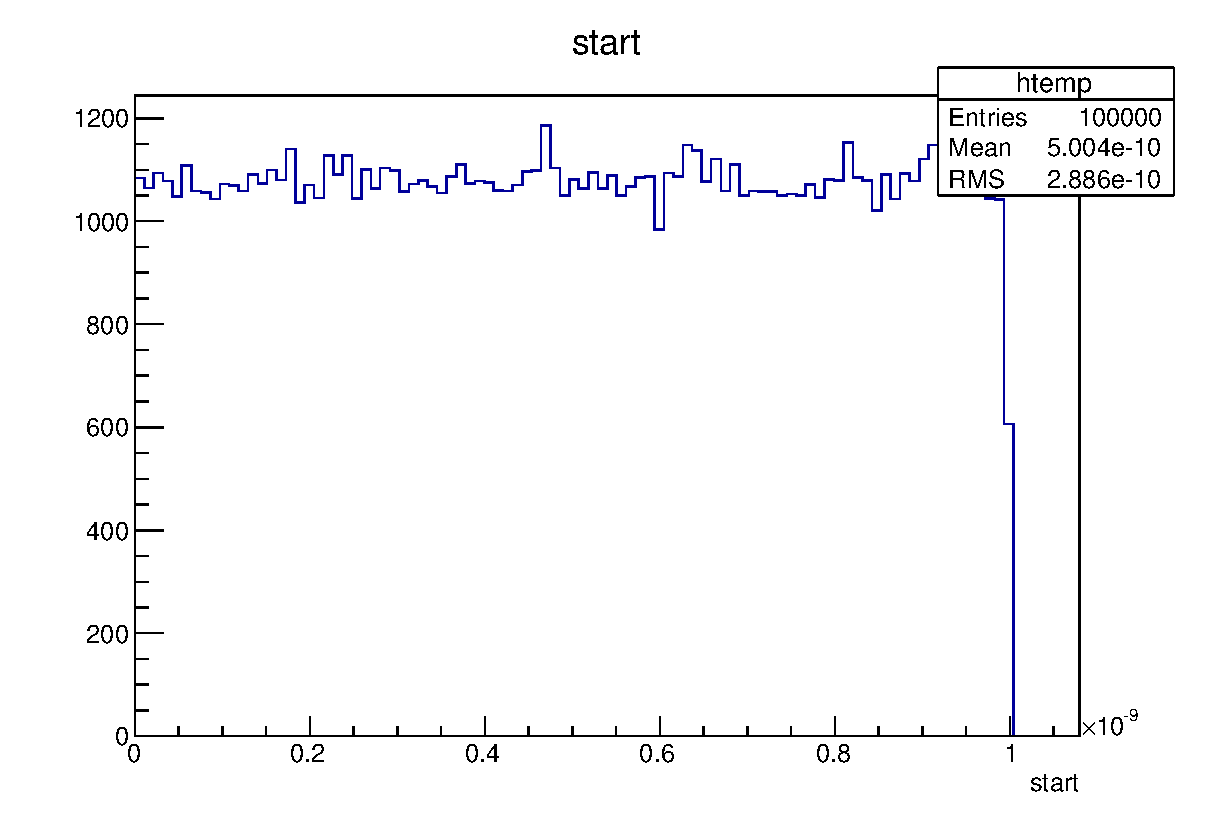
\includegraphics[width = 70mm]{./picture/meettreecanvas1.eps}
  \end{center}
  \caption{\texttt{tree->Draw("start")}実行によって表示される\texttt{start}のヒストグラム}
  \label{Fig:meettreecanvas1}
 \end{minipage}
 \begin{minipage}{0.45\hsize}
  \begin{center}
   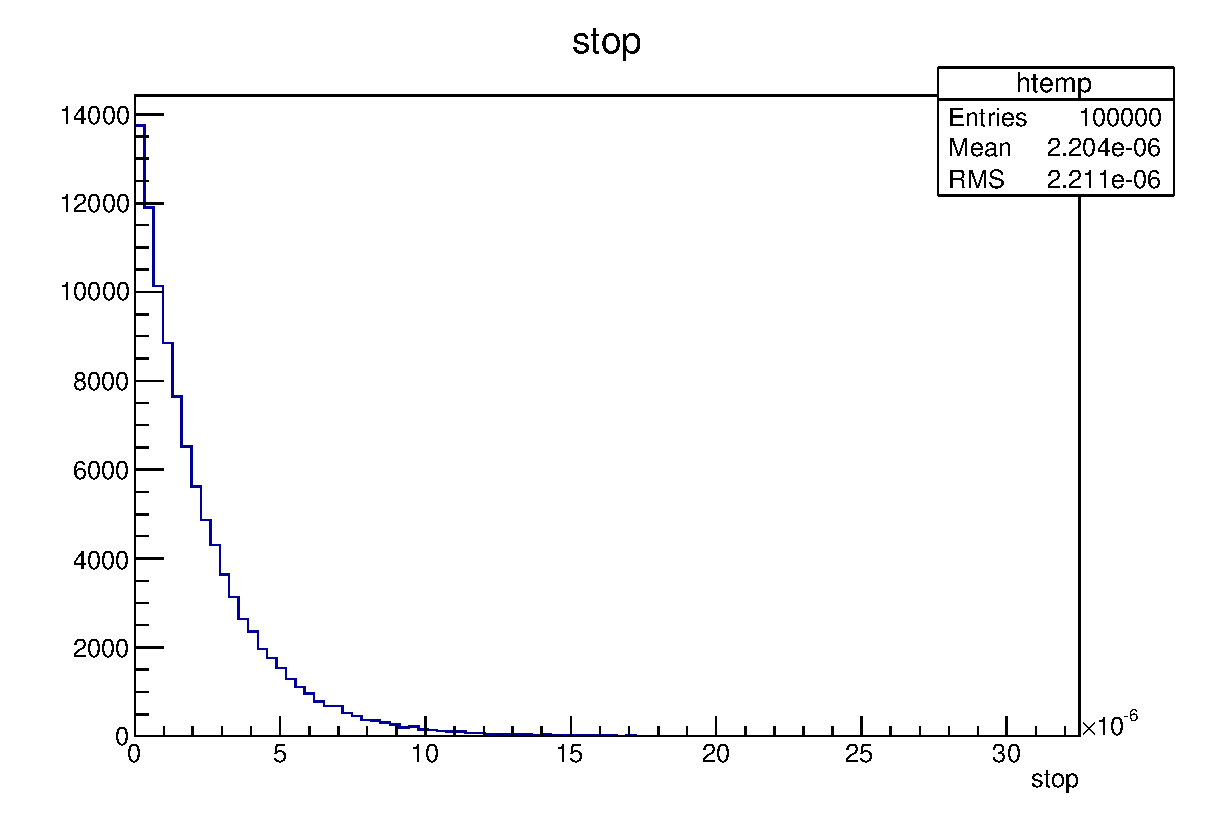
\includegraphics[width = 70mm]{./picture/meettreecanvas2.eps}
  \end{center}
  \caption{\texttt{tree->Draw("stop")}実行によって表示される\texttt{stop}のヒストグラム}
  \label{Fig:meettreecanvas2}
 \end{minipage}
\end{figure}


何もしなければbin数やヒストグラムの領域は自動で決まるが設定することももちろん出来る。
\begin{verbatim}
	root [5] tree->Draw("start>>h(100, 0., 1e-9)")
\end{verbatim}
などとすればわかるだろう。

  \subsection{練習}
  \begin{enumerate}
   \item コマンドライン上ででtdcの値格納用のヒストグラムのを用意した後、TDCのヒストグラムを描け。
	 \begin{description}
	  \item[ヒント] \url{http://root.cern.ch/root/html/TTree.html#TTree:Draw@2}
	 \end{description}
   \item tdcをx軸、startをy軸とした図\ref{Fig:meettreecanvas3}のような2次元ヒストグラムをコマンドラインから描け。
	 \begin{figure}[htbp]
	  \begin{center}
	   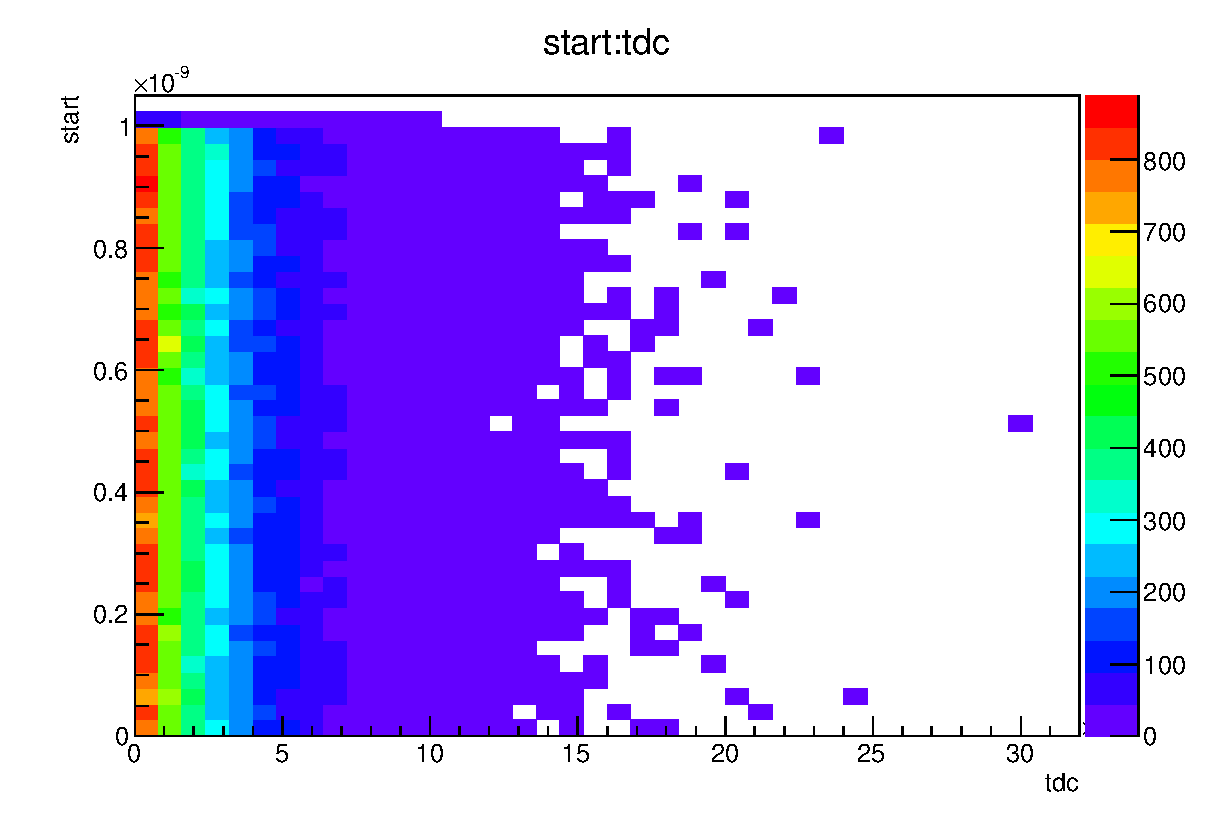
\includegraphics[width = 100mm]{./picture/meettreecanvas3.eps}
	  \end{center}
	  \caption{\texttt{start}実行によって表示される\texttt{start}のヒストグラム}
	  \label{Fig:meettreecanvas3}
	 \end{figure}


	 \begin{description}
	  \item[ヒント] \url{http://root.cern.ch/root/html/THistPainter.html#HP01c}
	 \end{description}
  \end{enumerate}

  \subsection{解答例}
  \begin{enumerate}
   \item コマンドライン上ででtdcの値格納用のヒストグラムのを用意した後、TDCのヒストグラムを描け。
\begin{verbatim}
	root [] TH1D *h = new TH1D("h", "h", 100, 0., 8000e-9)
	root [] tree->Draw("tdc>>h")
	Info in <TCanvas::MakeDefCanvas>:  created default TCanvas with name c1
\end{verbatim}
   \item tdcをx軸、startをy軸とした図\ref{Fig:meettreecanvas3}のような2次元ヒストグラムをコマンドラインから描け。
\begin{verbatim}
	root [] tree->Draw("start:tdc","","colz")
\end{verbatim}
  \end{enumerate}


  %%%%%%%%%%%%%%%%%%%%%%%%%%%%%%%%%%%%%%%%%%%%%%%%%%%%%%%%%%%%%%%%%%%%%%%%%%%%%%%%%
  %%        %%%        %%%        %%%        %%%        %%%         %%%  %%%%  %%%
  %%  %%%%%%%%%  %%%%%%%%%  %%%%%%%%%%%%  %%%%%%%%%  %%%%%%  %%%%%  %%%    %%  %%%
  %%        %%%        %%%  %%%%%%%%%%%%  %%%%%%%%%  %%%%%%  %%%%%  %%%  %  %  %%%
  %%%%%%%%  %%%  %%%%%%%%%  %%%%%%%%%%%%  %%%%%%%%%  %%%%%%  %%%%%  %%%  %%    %%%
  %%        %%%        %%%        %%%%%%  %%%%%%        %%%         %%%  %%%   %%%
  %%%%%%%%%%%%%%%%%%%%%%%%%%%%%%%%%%%%%%%%%%%%%%%%%%%%%%%%%%%%%%%%%%%%%%%%%%%%%%%%%
 \section{Treeから読んで描く}

 \begin{itembox}{\texttt{meettree2.cpp}}
\begin{verbatim}
	#include "TCanvas.h"
	#include "TFile.h"
	#include "TH1D.h"
	#include "TTree.h"

	TH1D *meettree2(char *InputRootFileName){

	TCanvas *c1 = new TCanvas("c1", "c1") ;
	TFile *file = new TFile(InputRootFileName,"READ") ;
	TTree *t = (TTree*)file->Get("tree") ;

	TH1D *h = new TH1D("h","TDC",100, 0., 8000e-9) ; // 8000[ns]
	t->Draw("tdc>>h") ;

	c1->cd() ;
	h->Draw() ;

	return h ;
	}
\end{verbatim}
 \end{itembox}


  \subsection{練習}
  \begin{enumerate}
   \item プログラムの挙動を理解せよ。
	 \begin{description}
	  \item[ヒント] \url{http://root.cern.ch/root/html/TFile.html#TFile:TFile@2}
	  \item[ヒント] \url{http://root.cern.ch/root/html/TDirectoryFile.html#TDirectoryFile:Get}
	 \end{description}
   \item これまでの知識を動員して、\verb|meettree2.cpp|を改良せよ。
	 具体的には軸に単位を追加したり、
	 自動的にFitしたりするなどせよ。
  \end{enumerate}

  \subsection{解答例}


\chapter{ネイティブプログラミング}

  %%%%%%%%%%%%%%%%%%%%%%%%%%%%%%%%%%%%%%%%%%%%%%%%%%%%%%%%%%%%%%%%%%%%%%%%%%%%%%%%%
  %%        %%%        %%%        %%%        %%%        %%%         %%%  %%%%  %%%
  %%  %%%%%%%%%  %%%%%%%%%  %%%%%%%%%%%%  %%%%%%%%%  %%%%%%  %%%%%  %%%    %%  %%%
  %%        %%%        %%%  %%%%%%%%%%%%  %%%%%%%%%  %%%%%%  %%%%%  %%%  %  %  %%%
  %%%%%%%%  %%%  %%%%%%%%%  %%%%%%%%%%%%  %%%%%%%%%  %%%%%%  %%%%%  %%%  %%    %%%
  %%        %%%        %%%        %%%%%%  %%%%%%        %%%         %%%  %%%   %%%
  %%%%%%%%%%%%%%%%%%%%%%%%%%%%%%%%%%%%%%%%%%%%%%%%%%%%%%%%%%%%%%%%%%%%%%%%%%%%%%%%%
 \section{ネイティブプログラムへの移行準備}

 \subsection{プログラミング言語とコンパイラ}
 とりあえず動かすことを目的としてきたので、
 一旦落ち着いてコンパイラの話をする。

 今まで我々が扱ってきたソースコードは全て人間のための言葉であり、
 機械のための言葉ではない。
 このような言語を高水準言語と呼ぶ。
 一方、機会が実際に実行できる仕様になっている言語のことを低水準言語または機械語などと言ったりする。
 プログラマが書いた高水準言語を低水準言語に変換してくれるのがコンパイラである。
 
 
  \subsection{コンパイラ \texttt{c++}}
  \Cpp 用のコンパイラ。
  本テキストでは コンパイラとして\texttt{c++}を常に用いる。
  
  
  \subsection{コンパイルする}
  
  サンプルプログラム\texttt{hello2.cpp}をコンパイルする方法を紹介する。
  \begin{itembox}{\texttt{hello2.cpp}}
\begin{verbatim}
#include <iostream>
int main(int argc, char** argv){
  std::cout << "Hello, World" << std::endl;
  return EXIT_SUCCESS ;
}
\end{verbatim}
  \end{itembox}
   
   
   \subsubsection*{一番シンプルなコンパイル}
   \begin{verbatim}
	$ c++ hello2.cpp
   \end{verbatim}
   これで\texttt{a.out}が出来上がる。
   この\texttt{a.out}が実行ファイルである。
   実行ファイルを実行する方法は
   \begin{verbatim}
	$ ./a.out
	Hello, World
   \end{verbatim}
   
   
   \subsubsection*{実行ファイルの名前を指定してコンパイル}
   実行ファイル名を\texttt{a.out}以外にしたい時には\verb|-o|オプションを用いる。
   \begin{verbatim}
	c++ hello2.cpp -o hello2
   \end{verbatim}
   これで実行ファイル\texttt{hello2}が生成される。
   実行方法は先の場合とファイル名が違うだけで
   \begin{verbatim}
	$ ./hello2
	Hello, World
   \end{verbatim}
   
   
   
   \subsubsection*{全ての警告文を表記するオプションを追加してコンパイル}
   コンパイル時にオプション\verb|-Wall|オプションを用いることで、
   コンパイラが警告できる警告文を全て表記させる事ができる。
   \begin{verbatim}
	c++ -Wall hello2.cpp -o hello2
   \end{verbatim}
   と言った具合である。
   
   試しにサンプルプログラム\texttt{hello2wrong.cpp}
  \begin{itembox}{\texttt{hello2wrong.cpp}}
\begin{verbatim}
#include <iostream>
int main(int argc, char** argv){
  std::cout << "Hello, World" << std::endl
  return EXIT_SUCCESS ;
}
\end{verbatim}
  \end{itembox}
  をコンパイルしてみると、下記のようなエラー文を返してくれる。
\begin{verbatim}
$c++ -Wall hello2wrong.cpp -o hello2wrong
hello2wrong.cpp: In function ‘int main(int, char**)’:
hello2wrong.cpp:4: error: expected `;' before ‘return’	
\end{verbatim}




\subsection{オブジェクトファイル}
初心者には更に厄介な事情がある。
今までは直接実行ファイルを作成していたが、
"関連してくるファイルが増えてきた時には、
各ソースコードからオブジェクトファイルと呼ばれるものを作成し、
オブジェクトファイルの組み合わせによって実行ファイルを作成する。"
というプロセスを得るのが普通である。
オプション\verb|-c|をつけることによって、
オブジェクトファイルを作成するところまでを行わせることが出来る。
  %%%%%%%%%%%%%%%%%%%%%%%%%%%%%%%%%%%%%%%%%%%%%%%%%%%%%%%%%%%%%%%%%%%%%%%%%%%%%%%%%
  %%        %%%        %%%        %%%        %%%        %%%         %%%  %%%%  %%%
  %%  %%%%%%%%%  %%%%%%%%%  %%%%%%%%%%%%  %%%%%%%%%  %%%%%%  %%%%%  %%%    %%  %%%
  %%        %%%        %%%  %%%%%%%%%%%%  %%%%%%%%%  %%%%%%  %%%%%  %%%  %  %  %%%
  %%%%%%%%  %%%  %%%%%%%%%  %%%%%%%%%%%%  %%%%%%%%%  %%%%%%  %%%%%  %%%  %%    %%%
  %%        %%%        %%%        %%%%%%  %%%%%%        %%%         %%%  %%%   %%%
  %%%%%%%%%%%%%%%%%%%%%%%%%%%%%%%%%%%%%%%%%%%%%%%%%%%%%%%%%%%%%%%%%%%%%%%%%%%%%%%%%
 \section{Makefileその1}
 
 

 \subsection{Make(メイク)}

 メイクとはMakefileと呼ばれるルールを記述したファイル、
 または予め定義された規則などからUNIXのShellが実行するコマンド列を作成するコマンドジェネレータの役目を持つ。
 メイクはファイル間の依存関係を整理するのにも使われ、大規模プログラミングでは必須のツールである。
 \verb|make|というコマンドがまず自分のPCに導入されているかを確認しておいて欲しい。
 なければどこぞからインストールしてくること。
 \verb|make|があるかどうかの確認は
 \begin{verbatim}
	$ which make
	/usr/bin/make
 \end{verbatim}
\verb|make|のヴァージョン確認は
 \begin{verbatim}
	$ make -v
GNU Make 3.81
Copyright (C) 2006  Free Software Foundation, Inc.
This is free software; see the source for copying conditions.
There is NO warranty; not even for MERCHANTABILITY or FITNESS FOR A
PARTICULAR PURPOSE.

This program built for i386-apple-darwin11.3.0
 \end{verbatim}
 
 
 
 \subsection{Makefile}
 Makefileメイクで実行するコマンド列を定義しておくファイル名である。
 Makefileが存在するディレクトリ下において、
 \begin{verbatim}
	$ make
 \end{verbatim}
 と入力することでMakefileにかかれた内容が実行される。
 なお、
 \verb|make|で実行したいファイル名が\verb|Makefile2|の場合には
 \begin{verbatim}
	$ make -f Makefile2
 \end{verbatim}
 \verb|make|で実行したいファイル名が\verb|hogex|の場合には
 \begin{verbatim}
	$ make -f hogex
 \end{verbatim}
 などとすればよい。
 
 
 \clearpage
 \subsection{直打ちメイクファイル}
まずは\texttt{hello2.cpp}を\verb|make|することで実行ファイルを作成するMakefileを作ってみよう。
お作法を知らなくてもまずは真似をして書いてみて欲しい。
\begin{itembox}{\texttt{Makefile}}
\begin{verbatim}
# Makefileの中では #で始まる行は実際にはコメントアウトされます。
# hello2.cppからhello2という実行ファイルを作成する為のMakefile
all:hello2

hello2:
        c++ -Wall hello2.cpp -o hello2
\end{verbatim}
\end{itembox}
ただし、\textcolor{red}{'\texttt{c++ -Wall hello2.cpp -o hello2}'の行の行頭は\texttt{<TAB>}を用いること。}

\texttt{hello2.cpp}と\texttt{Makefile}が同じディレクトリにいることを確認した後、
早速\verb|make|を実行し、
実行ファイル\texttt{hello2}が出来上がっていることを確認しよう。
\begin{verbatim}
	$ ls
Makefile	hello2.cpp
	$ make
c++     hello2.cpp   -o hello2
	$ ls
Makefile	hello2		hello2.cpp
\end{verbatim}


\subsubsection*{直打ちメイクファイルの解説}
\texttt{Makefile}の中身を順序立てて追っていく。
\begin{enumerate}
 \item \verb|all:hello2| \\
       コロン記号\verb|:|の直前の\verb|all|のことをターゲットという。
       \verb|make|を実行すると、デフォルトで\verb|all|というターゲットが存在するかどうかをチェックする。
       そして今は\verb|all|が定義されているので、
       この行が処理の対象となる。
       次にターゲットの右にリストされるターゲットから実行する。
       今の場合、\verb|hello2|がリストされているので、
       次のターゲットが\verb|hello2|ということになる。

 \item \verb|hello2:| \\
       ターゲットが\verb|hello2|を意味している。
       この行はターゲットの場所を顕に示しただけであり、
       すぐ次の文へと移る。
       
\item \verb|        c++ -Wall hello2.cpp -o hello2| \\
       ターゲットが\verb|hello2|に属している実行分である。
      \textcolor{red}{Makefileでは実行分の行頭を\texttt{<TAB>}でインデントする必要があるので注意すること。}
      この文で実行される内容は、\verb|hello2.cpp|というソースコードをコンパイルして、
      実行ファイル\verb|hello2|を作るという動作である。
\end{enumerate}



\clearpage
 \subsection{マクロを利用したメイクファイル}
 直打ちメイクファイルはかっこ悪いので少しずつランクアップをしよう。
 \texttt{Makefile}ではマクロという変数を用いることで、
 直打ちから脱却が出来る。
 その例が\texttt{Makefike2}である。
  %%%%%%%%%%%%%%%%%%%%%%%%%%%%%%%%%%%%%%%%%%%%%%%%%%%%%%%%%%%%%%%%%%%%%%%%%%%%%%%%%
  %%        %%%        %%%        %%%        %%%        %%%         %%%  %%%%  %%%
  %%  %%%%%%%%%  %%%%%%%%%  %%%%%%%%%%%%  %%%%%%%%%  %%%%%%  %%%%%  %%%    %%  %%%
  %%        %%%        %%%  %%%%%%%%%%%%  %%%%%%%%%  %%%%%%  %%%%%  %%%  %  %  %%%
  %%%%%%%%  %%%  %%%%%%%%%  %%%%%%%%%%%%  %%%%%%%%%  %%%%%%  %%%%%  %%%  %%    %%%
  %%        %%%        %%%        %%%%%%  %%%%%%        %%%         %%%  %%%   %%%
  %%%%%%%%%%%%%%%%%%%%%%%%%%%%%%%%%%%%%%%%%%%%%%%%%%%%%%%%%%%%%%%%%%%%%%%%%%%%%%%%%
 \section{Makefileその2:ファイルを分割する}
 
 
 

整数の3乗を計算するプログラム\texttt{cube.cpp}を分割することを考える。
\begin{itembox}{\texttt{cube.cpp}}
 \begin{verbatim}
#include "iostream"
int cube(int a) ;

int main(int argc, char** argv){
  std::cout << cube(4) << std::endl ;
  return EXIT_SUCCESS ;
}

int cube(int a){
  return a*a*a ;
}
 \end{verbatim}
\end{itembox}
この時のメイクファイルは
\begin{itembox}{\texttt{Makefile}}
\begin{verbatim}
TARGET = cube
COM    = c++
CFLAGS = -Wall
OBJS   = $(TARGET).o

all:$(TARGET)

$(TARGET):$(OBJS)
	$(COM) $(CFLAGS) $(TARGET).cpp -o $^
$(OBJS):$(TARGET).cpp
	$(COM) -c $<

clean:
        rm -f *.o
\end{verbatim}
\end{itembox}
	
	
	
\clearpage
 \subsection{分割したファイルのコンパイル}

ファイルを次の三つに分割する。
\begin{itembox}{\texttt{head.h}}
\begin{verbatim}
int cube(int) ;
\end{verbatim}
\end{itembox}

\begin{itembox}{\texttt{sub.cpp}}
\begin{verbatim}
#include "head.h"
int cube(int a){
  return a*a*a ;
}
\end{verbatim}
\end{itembox}

\begin{itembox}{\texttt{main.cpp}}
\begin{verbatim}
#include "head.h"
#include <iostream>
int cube(int a) ;

int main(int argc, char** argv){
  std::cout << cube(4) << std::endl ;
  return EXIT_SUCCESS ;
}
\end{verbatim}
\end{itembox}

これら三つのファイルをつかったコンパイルの方法は柿の通りである。
\begin{verbatim}
$ ls
head.h		main.cpp	sub.cpp
$ c++ -c main.cpp
$ c++ -c sub.cpp
$ ls
head.h		main.cpp	main.o		sub.cpp		sub.o
$ c++ -o main main.o sub.o
$ ls
head.h		main		main.cpp	main.o		sub.cpp		sub.o
\end{verbatim}
また、
これらの動作をひと綴りにした\texttt{Makefile}を\texttt{Makefile2}に示す。
\begin{itembox}{\texttt{Makefile2}}
 \begin{verbatim}
TARGET = main
TARGET2= sub
HEAD   = head

COM    = c++
CFLAGS = -Wall
OBJS   = $(TARGET).o $(TARGET2).o

all:$(TARGET)

$(TARGET):$(OBJS)
        $(COM) $(CFLAGS) -o $(TARGET) $(OBJS)

$(TARGET).o:$(TARGET).cpp $(HEAD).h
        $(COM) -c $<

$(TARGET2).o:$(TARGET2).cpp $(HEAD).h
        $(COM) -c $<
clean:
        rm -f *.o
 \end{verbatim}
\end{itembox}
\texttt{Makefile2}の使い方は下記の通り、
\begin{verbatim}
$ make -f Makefile2
c++ -c main.cpp
c++ -c sub.cpp
c++ -Wall -o main main.o sub.o
$ ./main
64
\end{verbatim}


\begin{itembox}{\texttt{Makefile3}}
 \begin{verbatim}
TARGET = main
TARGET2= sub
HEAD   = head

COM    = c++
CFLAGS = -Wall
OBJS   = $(TARGET).o $(TARGET2).o

all:$(TARGET)

$(TARGET):$(OBJS)
        $(COM) $(CFLAGS) -o $(TARGET) $(OBJS)
.cpp.o:
        $(CC) $(CFLAGS) -c $<
$(TARGET).o : $(HEAD).h  # main.cppの依存ファイルは head.h
$(TARGET2).o: $(HEAD).h # main.cppの依存ファイルは head.h

clean:
        rm -f *.o\end{verbatim}
\end{itembox}
\texttt{Makefile3}の使い方は下記の通り、
\begin{verbatim}
$ make -f Makefile3
c++ -c main.cpp
c++ -c sub.cpp
c++ -Wall -o main main.o sub.o
$ ./main
64
\end{verbatim}
%%%%%%%%%%%%%%%%%%%%%%%%%%%%%%%%%%%%%%%%%%%%%%%%%%%%%%%%%%%%%%%%%%%%%%%%%%%%%%%%%
%%        %%%        %%%        %%%        %%%        %%%         %%%  %%%%  %%%
%%  %%%%%%%%%  %%%%%%%%%  %%%%%%%%%%%%  %%%%%%%%%  %%%%%%  %%%%%  %%%    %%  %%%
%%        %%%        %%%  %%%%%%%%%%%%  %%%%%%%%%  %%%%%%  %%%%%  %%%  %  %  %%%
%%%%%%%%  %%%  %%%%%%%%%  %%%%%%%%%%%%  %%%%%%%%%  %%%%%%  %%%%%  %%%  %%    %%%
%%        %%%        %%%        %%%%%%  %%%%%%        %%%         %%%  %%%   %%%
%%%%%%%%%%%%%%%%%%%%%%%%%%%%%%%%%%%%%%%%%%%%%%%%%%%%%%%%%%%%%%%%%%%%%%%%%%%%%%%%%
 \section{Makefileその3:引数を利用する}
 
 
 ファイルを実行する時に引数を与えたくなるだろう。
 その簡単な方法を示す。
 いままでおまじないとして
 \verb|main|の引数に\verb|int|型の\verb|argc|、\verb|char**|型の\verb|argv|を記入していた。
 \begin{itemize}
  \item \verb|argc| \\
	実行ファイル$+$与えた引数の数を表す。 \\
	引数が0ならば\verb|argc=1|、
	引数が1つならば\verb|argc=2|、
	引数が2つならば\verb|argc=3|、
	
  \item \verb|argv| \\
	与えた引数を文字列として格納している。\\
	\verb|argv[0]|は実行ファイル名、
	\verb|argv[1]|は第1引数、
	\verb|argv[2]|は第2引数といった具合である。
 \end{itemize}
 
 
 
  \subsection{とりあえず動かす}
  
  引数の数と引数の文字列を表記するサンプルプログラム\texttt{show.cpp}と、
  その\texttt{Makefile}を次に示す。
  \begin{itembox}{\texttt{show.cpp}}
\begin{verbatim}
#include <iostream>
int main(int argc,char** argv){
  std::cout << "argc = " << argc << std::endl ;
  for(int i=0; i< argc ;i++){
    std::cout << "argv[" << i << "]= " << argv[i] << std::endl;
  }
  return EXIT_SUCCESS ;
}
\end{verbatim}
  \end{itembox}
  
  \begin{itembox}{\texttt{Makefile}}
\begin{verbatim}
TARGET = show

COM    = c++
CFLAGS = -Wall
OBJS   = $(TARGET).o

all:$(TARGET)

$(TARGET):$(OBJS)
	$(COM) $(CFLAGS) -o $(TARGET) $(OBJS)
.cpp.o:
	$(CC) $(CFLAGS) -c $<
$(TARGET).o :

clean:
	rm -f *.o
\end{verbatim}
  \end{itembox}
  
  実行例は次のとおりである。
  まずは\verb|make|。
\begin{verbatim}
$ ls	
Makefile	show.cpp
$ make
cc -Wall -c show.cpp
c++ -Wall -o show show.o
\end{verbatim}
次に引数を与えずに実行してみよう。
\begin{verbatim}
$ ./show
argc = 1
argv[0]= ./show
\end{verbatim}
引数を与えていないので、
\verb|argc|は実行ファイルのみをしめす$1$、
\verb|argv[0]|は今実行した実行ファイル名になっている。

次に引数を3つ与えてみる。
\begin{verbatim}
$ ./show a b c
argc = 4
argv[0]= ./show
argv[1]= a
argv[2]= b
argv[3]= c
\end{verbatim}
verb|argc|は実行ファイル以外に3つの引数を持つことを示す$4$、
\verb|argv[i]|はそれぞれ実行ファイル名を引数に対応する文字列である。

文字列の大きさは1文字でなくても良い。
\begin{verbatim}
$ ./show abc
argc = 2
argv[0]= ./show
argv[1]= abc
\end{verbatim}

数字を引数に与えてみるとどうなるだろうか?
\begin{verbatim}
$ ./show a. 1.e-2
argc = 3
argv[0]= ./show
argv[1]= a.
argv[2]= 1.e-2
\end{verbatim}
ここで注意して欲しいのは、
\verb|argv[2]|は文字列として出力されているということだ。
例えば\ROOT のコマンドライン上で\verb|1.e-2|を入力すると、
\begin{verbatim}
root [] 1.e-2
(const double)1.00000000000000002e-02
\end{verbatim}
と表示されるが、先ほどの例では入力した文字列のままで出力されていることに注意しておく必要が有る。
したがって、\textcolor{red}{\texttt{argv[i]}を数字として直接扱うことはバグの原因となりえる}ので注意すること。
\verb|argv[i]|を数字に変換する方法は練習問題とする。

\subsection{練習}

\begin{enumerate}
 \item 実行ファイル自身以外の引数の数が2以外だとエラーメッセージを返すようにせよ。
       
 \item 2つの引数の和を表示するように変更せよ。
       ただし、入力される引数は数字だけが入力されると仮定してよい。
       (より応用な問題としては、そもそも引数が数字かどうかの判定なども考えられる。
       興味に応じて調べよ。)
       \begin{description}
	\item[ヒント] \url{http://www.cplusplus.com/reference/cstdlib/atof/}
       \end{description}
\end{enumerate}


\subsection{解答例}

\begin{enumerate}
 \item 実行ファイル自身以外の引数の数が2以外だとエラーメッセージを返すようにせよ。
       
 \item 2つの引数の和を表示するように変更せよ。
       ただし、入力される引数は数字だけが入力されると仮定してよい。
\end{enumerate}
\begin{itembox}{\texttt{showsol1.cpp}}
 \begin{verbatim}
#include <iostream>
int main(int argc,char** argv){
  std::cout << "argc = " << argc << std::endl ;
  if(argc!=3){
    std::cerr << "Usage like ... \n ./showsol1 3.2 4" << std::endl ;
    return EXIT_FAILURE ;
  }
  for(int i=0; i< argc ;i++){
    std::cout << "argv[" << i << "]= " << argv[i] << std::endl;
  }
  std::cout << argv[1] << " + " << argv[2] << " = " << atof(argv[1]) + atof(argv[2]) << std::endl;
  return EXIT_SUCCESS ;
}
 \end{verbatim}
\end{itembox}

実行結果は下記の通りである。
\begin{verbatim}
$ ./showsol1 
argc = 1
Usage like ... 
 ./showsol1 3.2 4
$ ./showsol1 6 4
argc = 3
argv[0]= ./showsol1
argv[1]= 6
argv[2]= 4
6 + 4 = 10
\end{verbatim}
%%%%%%%%%%%%%%%%%%%%%%%%%%%%%%%%%%%%%%%%%%%%%%%%%%%%%%%%%%%%%%%%%%%%%%%%%%%%%%%%%
%%        %%%        %%%        %%%        %%%        %%%         %%%  %%%%  %%%
%%  %%%%%%%%%  %%%%%%%%%  %%%%%%%%%%%%  %%%%%%%%%  %%%%%%  %%%%%  %%%    %%  %%%
%%        %%%        %%%  %%%%%%%%%%%%  %%%%%%%%%  %%%%%%  %%%%%  %%%  %  %  %%%
%%%%%%%%  %%%  %%%%%%%%%  %%%%%%%%%%%%  %%%%%%%%%  %%%%%%  %%%%%  %%%  %%    %%%
%%        %%%        %%%        %%%%%%  %%%%%%        %%%         %%%  %%%   %%%
%%%%%%%%%%%%%%%%%%%%%%%%%%%%%%%%%%%%%%%%%%%%%%%%%%%%%%%%%%%%%%%%%%%%%%%%%%%%%%%%%
 \section{Makefileその4:\ROOT のネイティブプログラミング}
 
 
 
 本章で\ROOT のライブラリなどネイティブでも使用できるようにする。
 
  \subsection{\ROOT ライブラリとのリンク}
  
  \ROOT の数式ライブラリに含まれている定義値$\pi$を表示しよう。
  \begin{itembox}{\texttt{pi.cpp}}
\begin{verbatim}
#include "TMath.h"
#include <iostream>
int main(int argc, char** argv){
  std::cout << "Pi = " << TMath::Pi() << std::endl ;
  return EXIT_SUCCESS ;
}
\end{verbatim}
  \end{itembox}
  メイクファイルを今までと同じように準備してみよう。
  \begin{itembox}{\texttt{pi.cpp}}
\begin{verbatim}
TARGET = pi

COM    = c++
CFLAGS = -Wall
OBJS   = $(TARGET).o

all:$(TARGET)

$(TARGET):$(OBJS)
        $(COM) $(CFLAGS) -o $(TARGET) $(OBJS)
.cpp.o:
        $(CC) $(CFLAGS) -c $<
$(TARGET).o :

clean:
        rm -f *.o
\end{verbatim}
  \end{itembox}
  
  
  \verb|make|を実行してみると、
\begin{verbatim}
$ make
cc -Wall -c pi.cpp
pi.cpp:1:10: fatal error: 'TMath.h' file not found
#include "TMath.h"
         ^
1 error generated.
make: *** [pi.o] Error 1
\end{verbatim}
はい、エラーが出ました。
そこで\texttt{Makefile}を次のように書き換える。
\begin{itembox}{\texttt{Makefile2}}
 \begin{verbatim}
TARGET = pi

COM        = c++
CFLAGS     = -Wall
ROOTCFLAGS = $(shell root-config --cflags)
ROOTLIBS   = $(shell root-config --libs)
CXXFLAGS   = $(ROOTCFLAGS) $(CFLAGS)
CXXLIBS    = $(ROOTLIBS)

OBJS   = $(TARGET).o

all:$(TARGET)

$(TARGET):$(OBJS)
	$(COM) $(CXXLIBS) -o $(TARGET) $(OBJS)
.cpp.o:
	$(CC) $(CXXFLAGS) -c $<
$(TARGET).o :

clean:
	rm -f *.o
 \end{verbatim}
\end{itembox}
行った変更はコンパイルフラグを追加したことと、
\ROOT のライブラリとのリンク作業である。
\verb|make|してみよう。
\begin{verbatim}
$ make -f Makefile2
cc -pthread -m64 -I/usr/local/hep/root/v5.34.09/include/root -Wall -c pi.cpp
c++ -L/usr/local/hep/root/v5.34.09/lib/root -lCore -lCint -lRIO -lNet -lHist \
-lGraf -lGraf3d -lGpad -lTree -lRint -lPostscript -lMatrix -lPhysics -lMathCore \
-lThread -lpthread -lm -ldl -o pi pi.o
$ ./pi 
Pi = 3.14159
\end{verbatim}
ちょっと長ったらしい実行分の後、
目的の実行ファイル\texttt{pi}が出来上がる。


\subsection{幾つかのサンプルプログラム}


   \subsubsection{ヒストグラムの描写と保存}
     \begin{itembox}{\texttt{hist2.cpp}}
\begin{verbatim}
#include "TCanvas.h"
#include "TH1.h"
#include <iostream>

int main(int argc, char** argv){
  TCanvas *c1 = new TCanvas("c1", "c1", 600, 600) ;
  TH1D *h = new TH1D("h", "h", 100, -5., 5.) ;
  h->FillRandom("gaus") ;
  h->Draw("E") ;
  c1->SaveAs("hist2c1.eps") ;
  delete h ;
  delete c1 ;
  return EXIT_SUCCESS ;
}
\end{verbatim}
     \end{itembox}

     \begin{itembox}{\texttt{Makefile}}
\begin{verbatim}
TARGET = hist2

COM        = c++
CFLAGS     = -Wall
ROOTCFLAGS = $(shell root-config --cflags)
ROOTLIBS   = $(shell root-config --libs)
CXXFLAGS   = $(ROOTCFLAGS) $(CFLAGS)
CXXLIBS    = $(ROOTLIBS)

OBJS   = $(TARGET).o

all:$(TARGET)

$(TARGET):$(OBJS)
        $(COM) $(CXXLIBS) -o $(TARGET) $(OBJS)
.cpp.o:
        $(CC) $(CXXFLAGS) -c $<
$(TARGET).o :

clean:
        rm -f *.o
\end{verbatim}
     \end{itembox}
     実行方法は下記の通り。
\begin{verbatim}
$ ls
Makefile	hist2.cpp
$ make
cc -pthread -m64 -I/usr/local/hep/root/v5.34.09/include/root -Wall -c hist2.cpp
c++ -L/usr/local/hep/root/v5.34.09/lib/root -lCore -lCint -lRIO -lNet -lHist -lGraf \
-lGraf3d -lGpad -lTree -lRint -lPostscript -lMatrix -lPhysics -lMathCore -lThread -lpthread \
 -lm -ldl -o hist2 hist2.o
$ ./hist2 
Info in <TCanvas::Print>: eps file hist2c1.eps has been created
$ ls
Makefile	hist2c1.eps		hist2		hist2.cpp	hist2.o
\end{verbatim}

     
   \subsubsection{}

     \begin{itembox}{\texttt{}}
\begin{verbatim}
\end{verbatim}
     \end{itembox}
     \begin{itembox}{\texttt{}}
\begin{verbatim}
\end{verbatim}
     \end{itembox}
   
   
   \subsubsection{}
   
        \begin{itembox}{\texttt{}}
\begin{verbatim}
\end{verbatim}
     \end{itembox}
     \begin{itembox}{\texttt{}}
\begin{verbatim}
\end{verbatim}
     \end{itembox}


\clearpage
\appendix

 %%%%%%%%%%%%%%%%%%%%%%%%%%%%%%%%%%%%%%%%%%%%%%%%%%%%%%%%%%%%%%%%%%%%%%%%%%%%%%%%%
 %%        %%%        %%%        %%%        %%%        %%%         %%%  %%%%  %%%
 %%  %%%%%%%%%  %%%%%%%%%  %%%%%%%%%%%%  %%%%%%%%%  %%%%%%  %%%%%  %%%    %%  %%%
 %%        %%%        %%%  %%%%%%%%%%%%  %%%%%%%%%  %%%%%%  %%%%%  %%%  %  %  %%%
 %%%%%%%%  %%%  %%%%%%%%%  %%%%%%%%%%%%  %%%%%%%%%  %%%%%%  %%%%%  %%%  %%    %%%
 %%        %%%        %%%        %%%%%%  %%%%%%        %%%         %%%  %%%   %%%
 %%%%%%%%%%%%%%%%%%%%%%%%%%%%%%%%%%%%%%%%%%%%%%%%%%%%%%%%%%%%%%%%%%%%%%%%%%%%%%%%%
 \section{名前空間\label{sec:namespace}}


 「あめ」といった時にそれがどういう内容を表すだろうか?
 識別する方法としては、
 \begin{enumerate}
  \item 「「気象現象」に属する「あめ」」
  \item「「食べ物」に属する「あめ」」
 \end{enumerate}
 などとしてしまえば、
 「あめ」の表す内容は明確になる。
 この時の「気象現象」や「食べ物」のようなくくりに当たる概念が名前空間である。
 この時使用した「属する」という言葉を\Cpp ではスコープ演算子\verb|"::"|で表す。
 つまり、先程の例を\Cpp 風に表現すると下記のようになる。
 \begin{enumerate}
  \item 気象現象\verb|::|あめ
  \item 食べ物\verb|::|あめ
 \end{enumerate}

  \subsection{名前空間\texttt{std::}}
  プログラム中で
\begin{verbatim}
	#include <iostream>
\end{verbatim}
と宣言すれば、
名前空間\texttt{std}が使用可能となる。
具体的な使い方としては、
\begin{verbatim}
	std::cout << "abc" << std::endl;
\end{verbatim}
などである。
意味としては、
\verb|abc|という文字列と\verb|std::endl|という改行命令を\verb|std::cout|で設定されている標準出力外面へ出力する。


  \subsection{名前空間\texttt{TMath::}}
  プログラム中で
\begin{verbatim}
	#include "TMath.h"
\end{verbatim}
と宣言すれば、
名前空間\texttt{TMath}が使用可能となる。
\url{http://root.cern.ch/root/html/TMath.html}
またコマンドライン上で\verb|ROOT|を使用する時には宣言の必要はない。
\begin{verbatim}
	root [] TMath::C()
	(Double_t)2.99792458000000000e+08
	root [] TMath::Pi()
	(Double_t)3.14159265358979312e+00
	root [] TMath::Power(2,3)
	(Double_t)8.00000000000000000e+00
	root [] TMath::Abs(-2.)
	(Double_t)2.00000000000000000e+00
	root [] TMath::Sin(1.)
	(Double_t)8.41470984807896505e-01
\end{verbatim}
などである。
上記の入力や引数や返り値の意味することは各自で調べよ。

%%%%%%%%%%%%%%%%%%%%%%%%%%%%%%%%%%%%%%%%%%%%%%%%%%%%%%%%%%%%%%%%%%%%%%%%%%%%%%%%%
%%        %%%        %%%        %%%        %%%        %%%         %%%  %%%%  %%%
%%  %%%%%%%%%  %%%%%%%%%  %%%%%%%%%%%%  %%%%%%%%%  %%%%%%  %%%%%  %%%    %%  %%%
%%        %%%        %%%  %%%%%%%%%%%%  %%%%%%%%%  %%%%%%  %%%%%  %%%  %  %  %%%
%%%%%%%%  %%%  %%%%%%%%%  %%%%%%%%%%%%  %%%%%%%%%  %%%%%%  %%%%%  %%%  %%    %%%
%%        %%%        %%%        %%%%%%  %%%%%%        %%%         %%%  %%%   %%%
%%%%%%%%%%%%%%%%%%%%%%%%%%%%%%%%%%%%%%%%%%%%%%%%%%%%%%%%%%%%%%%%%%%%%%%%%%%%%%%%%
 \section{\ROOT で使う色}

 \url{http://root.cern.ch/root/html/TAttFill.html#F1}
 \begin{figure}[htbp]
  \begin{center}
   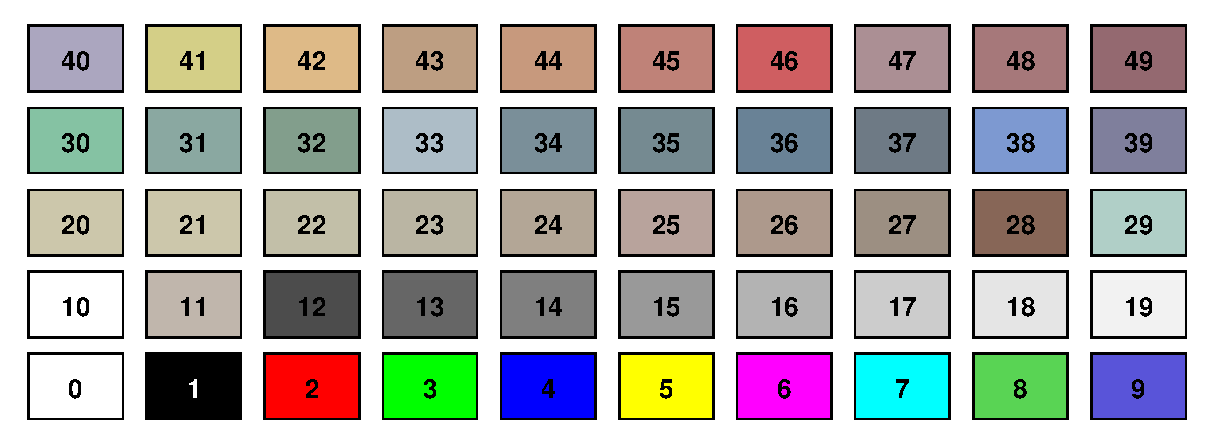
\includegraphics[width = 140mm]{./picture/filareacolor.eps}
  \end{center}
  \caption{\ROOT で使用できる色}
  \label{Fig:filareacolor}
 \end{figure}

 \begin{figure}[htbp]
  \begin{center}
   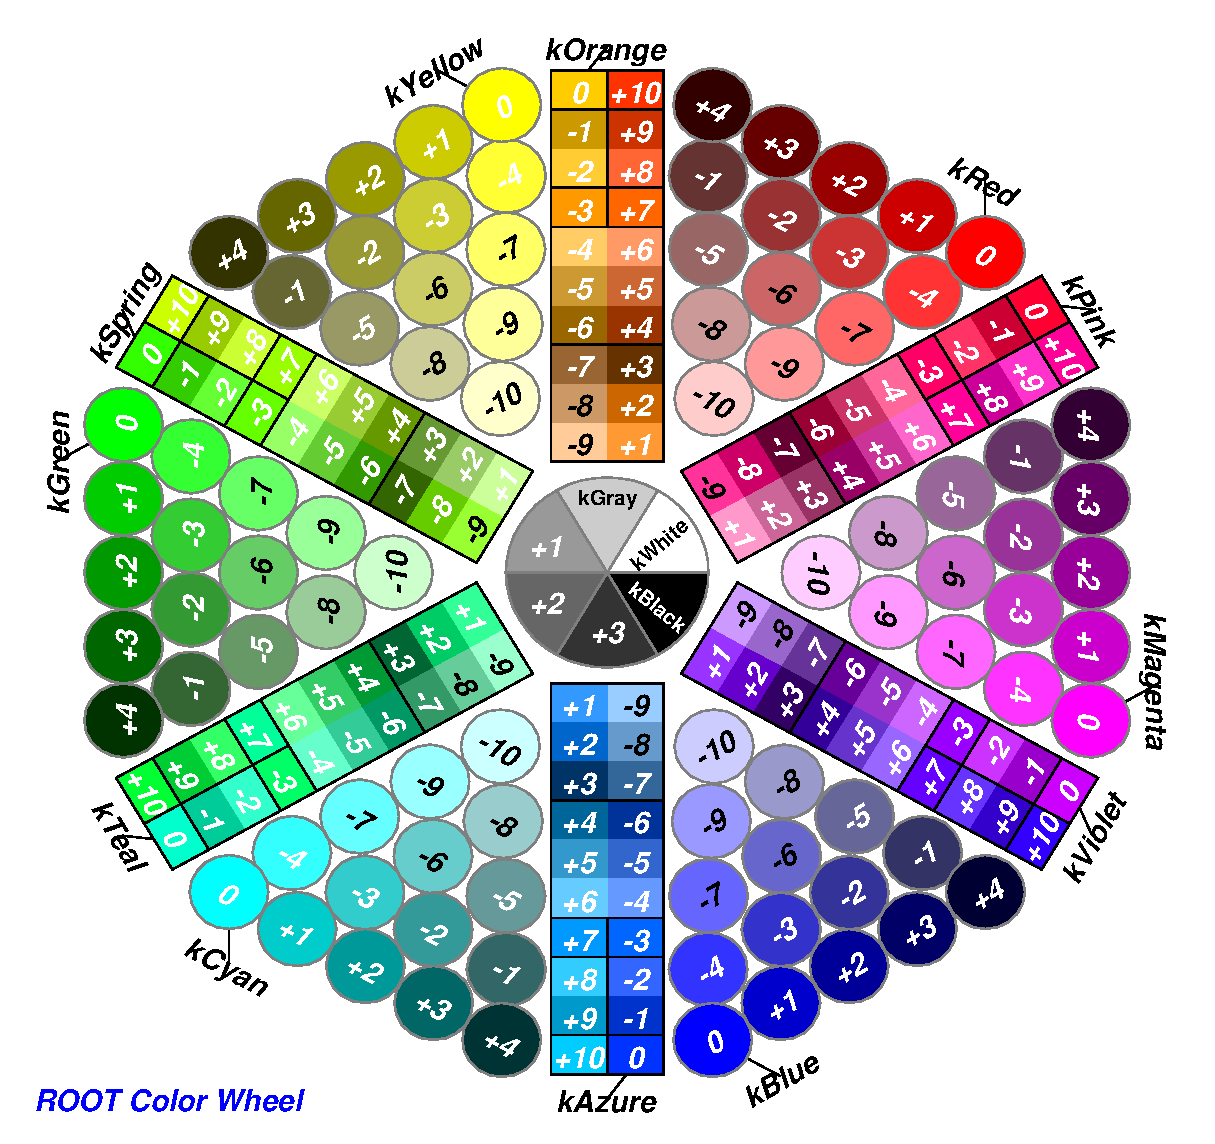
\includegraphics[width = 140mm]{./picture/rootcolorwheel.eps}
  \end{center}
  \caption{\ROOT で使用できる色}
  \label{Fig:rootcolorwheel}
 \end{figure}

 %%%%%%%%%%%%%%%%%%%%%%%%%%%%%%%%%%%%%%%%%%%%%%%%%%%%%%%%%%%%%%%%%%%%%%%%%%%%%%%%%
 %%        %%%        %%%        %%%        %%%        %%%         %%%  %%%%  %%%
 %%  %%%%%%%%%  %%%%%%%%%  %%%%%%%%%%%%  %%%%%%%%%  %%%%%%  %%%%%  %%%    %%  %%%
 %%        %%%        %%%  %%%%%%%%%%%%  %%%%%%%%%  %%%%%%  %%%%%  %%%  %  %  %%%
 %%%%%%%%  %%%  %%%%%%%%%  %%%%%%%%%%%%  %%%%%%%%%  %%%%%%  %%%%%  %%%  %%    %%%
 %%        %%%        %%%        %%%%%%  %%%%%%        %%%         %%%  %%%   %%%
 %%%%%%%%%%%%%%%%%%%%%%%%%%%%%%%%%%%%%%%%%%%%%%%%%%%%%%%%%%%%%%%%%%%%%%%%%%%%%%%%%

 \section{\ROOT で使うスタイル}

 \url{http://root.cern.ch/root/html/TAttFill.html#F2}
 \begin{figure}[htbp]
  \begin{center}
   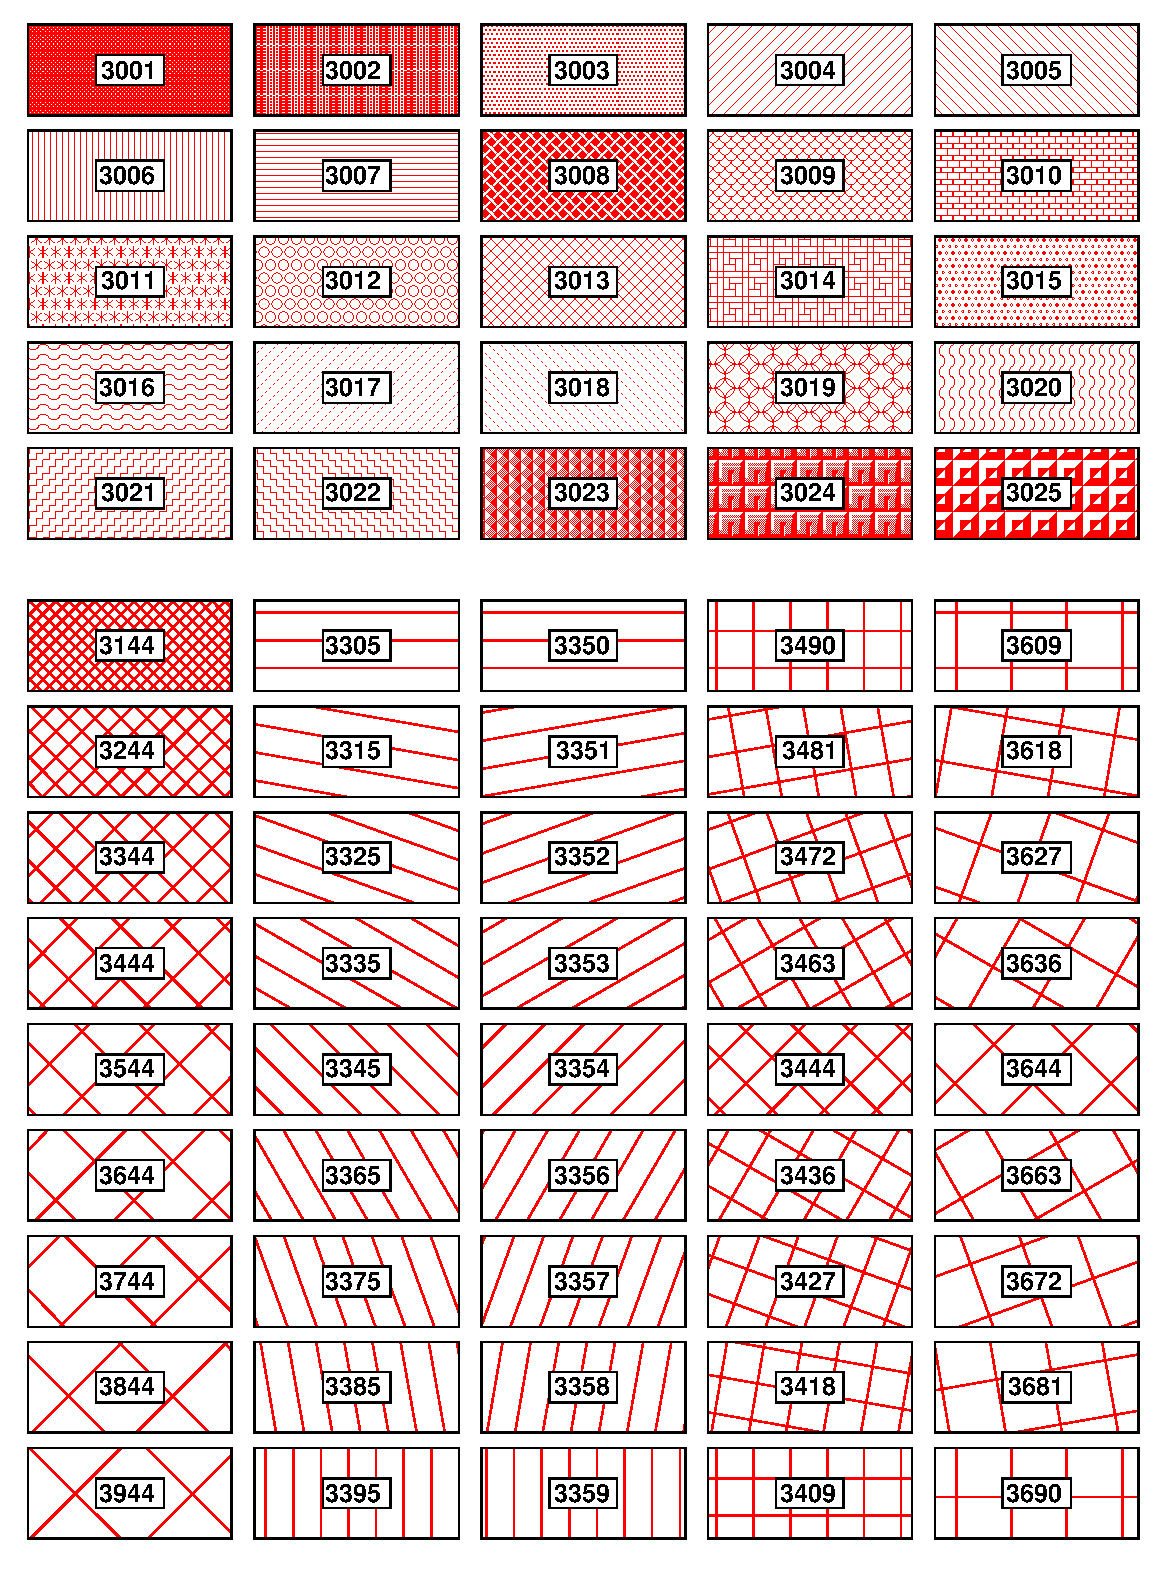
\includegraphics[height = 180mm]{./picture/fillpatterns.eps}
  \end{center}
  \caption{\ROOT で使用できるスタイル}
  \label{Fig:fillpatterns}
 \end{figure}


\end{document}